\documentclass[12pt]{article}

\usepackage{bm}
\usepackage{amsmath, mathtools}
\usepackage[justification=centering]{caption}
\usepackage{amsfonts}
\usepackage{amssymb}
\usepackage{commath}
\usepackage{graphicx}
\usepackage{pdflscape}
\usepackage{colortbl}
\usepackage{xr}
\usepackage{hyperref}
\usepackage{longtable}
\usepackage{xfrac}
\usepackage{tabularx}
\usepackage{float}
\usepackage[per-mode=reciprocal]{siunitx}
\usepackage{booktabs}

%\usepackage{refcheck}\underline{\underline{}}

\hypersetup{
    bookmarks=true,         % show bookmarks bar?
    colorlinks=true,       % false: boxed links; true: colored links
    linkcolor=red,          % color of internal links (change box color with linkbordercolor)
    citecolor=green,        % color of links to bibliography
    filecolor=magenta,      % color of file links
    urlcolor=cyan           % color of external links
}
\newcommand{\NN}[1]{{\color{red}#1}}
\newcommand{\WSS}[1]{{\color{blue}#1}}

\newcommand{\colZwidth}{1.0\textwidth}
\newcommand{\blt}{- } %used for bullets in a list
\newcommand{\colAwidth}{0.13\textwidth}
\newcommand{\colBwidth}{0.82\textwidth}
\newcommand{\colCwidth}{0.1\textwidth}
\newcommand{\colDwidth}{0.05\textwidth}
\newcommand{\colEwidth}{0.8\textwidth}
\newcommand{\colFwidth}{0.17\textwidth}
\newcommand{\colGwidth}{0.5\textwidth}
\newcommand{\colHwidth}{0.28\textwidth}
\newcounter{defnum} %Definition Number
\newcommand{\dthedefnum}{GD\thedefnum}
\newcommand{\dref}[1]{GD\ref{#1}}
\newcounter{datadefnum} %Datadefinition Number
\newcommand{\ddthedatadefnum}{DD\thedatadefnum}
\newcommand{\ddref}[1]{DD\ref{#1}}
\newcounter{theorynum} %Theory Number
\newcommand{\tthetheorynum}{T\thetheorynum}
\newcommand{\tref}[1]{T\ref{#1}}
\newcounter{tablenum} %Table Number
\newcommand{\tbthetablenum}{T\thetablenum}
\newcommand{\tbref}[1]{TB\ref{#1}}
\newcounter{assumpnum} %Assumption Number
\newcommand{\atheassumpnum}{P\theassumpnum}
\newcommand{\aref}[1]{A\ref{#1}}
\newcounter{goalnum} %Goal Number
\newcommand{\gthegoalnum}{P\thegoalnum}
\newcommand{\gsref}[1]{GS\ref{#1}}
\newcounter{instnum} %Instance Number
\newcommand{\itheinstnum}{IM\theinstnum}
\newcommand{\iref}[1]{IM\ref{#1}}
\newcounter{reqnum} %Requirement Number
\newcommand{\rthereqnum}{P\thereqnum}
\newcommand{\rref}[1]{R\ref{#1}}
\newcounter{lcnum} %Likely change number
\newcommand{\lthelcnum}{LC\thelcnum}
\newcommand{\lcref}[1]{LC\ref{#1}}
\newcommand{\dv}{\mathrm{d}\mathbf{v}}
\newcommand{\dx}{\mathrm{d}\mathbf{x}}
\newcommand{\dr}{\mathrm{d}\mathbf{r}}
\newcommand{\dpos}{\mathrm{d}\mathbf{p}}
\newcommand{\dt}{\mathrm{d}t}

\newcommand{\tclad}{T_\text{CL}}
\newcommand{\degree}{\ensuremath{^\circ}}
\newcommand{\progname}{Chipmunk2D}


\usepackage{fullpage}

\begin{document}

\title{Software Requirements Specification for Chipmunk2D} 
\author{Alex Halliwushka and Luthfi Mawarid}
\date{\today}
	
\maketitle

\tableofcontents

%% REVISION NOTES (31/5/2016)%%
% Tidied up the formatting of models and definitions to make it more readable and similar to other SRSs
% Revamped instance models
% Changed displacement symbol to r to avoid/minimize inconsistencies
% Added theta for angular displacement, changed center of mass to CM
% Changed 'damping coefficient' to 'damping ratio' - the former seems to 
% represent something slightly different

%%%%%%%%%%%%%%%%%%%%%%%%
%
%	1.) REFERENCE MATERIAL 
%
%%%%%%%%%%%%%%%%%%%%%%%%

\section{Reference Material}

This section records information for easy reference.


%1.1 Table of units
\subsection{Table of Units} \label{TblOfUnits}

Throughout this document, SI (Syst\`{e}me International d'Unit\'{e}s) is employed
as the unit system. For each unit, the symbol is given followed by a
description of the unit with the SI name. \\

\renewcommand{\arraystretch}{1.2}

  \noindent \begin{tabular}{l l l} 
    \toprule		
    \textbf{symbol} & \textbf{unit} & \textbf{SI}\\
    \midrule 
    \si{\meter} 	& length 		& meter\\
    \si{\kilogram}  & mass			& kilogram\\
    \si{\second} 	& time 			& second\\
    \si{\newton} 	& force 		& Newton\\
    \si{\radian} 	& angle 		& radians\\
    \bottomrule
  \end{tabular}


%1.2 Table of units
\subsection{Table of Symbols} \label{TblOfSym}

%%% NOTE: DECIDE IF SOME SYMBOLS NEED TO BE BOLDED

The table that follows summarizes the symbols used in this document along with
their units. More specific instances of these symbols will be described in their respective sections. Throughout the document, symbols in \textbf{bold} will represent vectors, and scalars otherwise. The symbols are listed in alphabetical order.

\renewcommand{\arraystretch}{1.2}
%\noindent \begin{tabularx}{1.0\textwidth}{l l X}
\noindent \begin{longtable}{l l p{12cm}} \toprule
  \textbf{symbol} & \textbf{unit} & \textbf{description}\\
  \midrule 
  $\mathbf{a}$ & \si{\metre\per\second\tothe{2}} & Acceleration \\
  $\alpha$ & \si{\radian\per\second\tothe{2}} & Angular acceleration \\
  $C_\text{R}$ & unitless & Coefficient of restitution \\
  $\mathbf{F}$ & \si{\newton} & Force \\
  $g$ & \si{\metre\per\second\tothe{2}} & Gravitational acceleration ($9.81$ \si{\metre\per\second\tothe{2}}) \\
  $G$ & \si{\metre\tothe{3}\per\kilogram\second\tothe{-2}} & Gravitational constant ($6.673 \times 10^{-11}$ \si{\metre\tothe{3}\per\kilogram\second\tothe{-2}}) \\
  $\mathbf{I}$ & \si{\kilogram\metre\tothe{2}} & Moment of inertia \\
  $\mathbf{\hat{i}}$ & \si{\metre} & Horizontal unit vector \\
  $\mathbf{\hat{j}}$ & \si{\metre} & Vertical unit vector \\
  $j$ & \si{\newton\second} & Impulse (scalar) \\
  $\mathbf{J}$ & \si{\newton\second} & Impulse (vector) \\
  %$\mathbf{k}$ & \si{\newton\per\metre} & Spring constant \\
  $L$ & \si{\metre} & Length \\
  $m$ & \si{\kilogram} & Mass \\
  $n$ & unitless & Number of particles in a rigid body \\
  $\mathbf{n}$ & \si{\metre} & Collision normal vector \\
  $\boldsymbol{\omega}$ & \si{\radian\per\second} & Angular velocity \\
  $\mathbf{p}$ & \si{\metre} & Position \\
  $\boldsymbol{\phi}$ & \si{\radian} & Orientation \\
  $r$ & \si{\metre} & Distance \\
  $\mathbf{r}$ & \si{\metre} & Displacement \\
  %$\mathbf{\rho}$ & \si{\kilogram\per\metre\tothe{3}} & Density \\
  $t$ & \si{\second} & Time \\
  $\tau$ & \si{\newton\metre} & Torque \\
  $\boldsymbol{\theta}$ & \si{\radian} & Angular displacement \\
  $\mathbf{v}$ & \si{\metre\per\second} & Velocity \\
  %$V$ & \si{\metre\tothe{3}} & Volume \\
  %$\mathbf{x}$ & \si{\metre} & Displacement of spring from equilibrium position \\
  \bottomrule
\end{longtable}

%1.3 Abbreviations and Acronyms
\subsection{Abbreviations and Acronyms}

\renewcommand{\arraystretch}{1.2}
\begin{tabular}{l l} 
  \toprule		
  \textbf{symbol} & \textbf{description}\\
  \midrule 
  A & Assumption\\
  CM & Center of Mass\\
  DD & Data Definition\\
  GD & General Definition\\
  GS & Goal Statement\\
  IM & Instance Model\\
  LC & Likely Change\\
  ODE & Ordinary Differential Equation\\
  R & Requirement\\
  SRS & Software Requirements Specification\\
  T & Theoretical Model\\
  2D & Two-dimensional \\
  \bottomrule
\end{tabular}\\

%% adding new page in case I need to add more symbols later

~\newpage

%%%%%%%%%%%%%%%%%%%%%%%%
%
%	2.) Introduction 
%
%%%%%%%%%%%%%%%%%%%%%%%%

\section{Introduction}

Due to the rising cost of developing video games, developers are looking for
ways to save time and money on their projects. Using an open source physics
library that is reliable and free will cut down development costs and lead 
to better quality products. \\
\newline
The following section provides an overview of the Software Requirements
Specification (SRS) for Chipmunk2D, an open source 2D rigid body physics library. It explains the purpose of this document,
the scope of the system, and the organization of the document.

%2.1 Purpose of Document

\subsection{Purpose of Document}

This document describes the modeling of an open source
2D rigid body physics library used for games. The goals and theoretical
models used in Chipmunk2D are provided. This document is intended to be 
used as a reference to provide all necessary information to understand and verify
the model. \\
\newline
This document will be used as a starting point for subsequent development
phases, including the writing of the design specification and the software verification
and validation plan. The design document will show how the requirements are 
to be realized. The verification and validation plan will show the steps that will 
be taken to increase confidence in the software documentation and 
implementation.

%2.2 Scope of Requirements
\subsection{Scope of Requirements} 

The scope of the requirements includes the physical simulation of 2D rigid bodies 
acted on by forces. Given 2D rigid bodies, Chipmunk2D is intended to 
simulate how these rigid bodies interact with one another.

%2.3 Organization of Document
\subsection{Organization of Document}
The organization of this document follows the template for an SRS for scientific
computing software proposed by~\cite{Koothoor2013} and \cite{SmithAndLai2005}.
The presentation follows the standard pattern of presenting goals, theories,
definitions, and assumptions.  For readers that would like a more bottom-up
approach, they can start reading the instance models in Section
\ref{sec_instance} and trace back to find any additional information they
require. \\
\newline
The goal statements are refined to the theoretical models, and theoretical
models to the instance models.  


%%%%%%%%%%%%%%%%%%%%%%%%
%
%	3.) General System Description
%
%%%%%%%%%%%%%%%%%%%%%%%%

\section{General System Description}

This section provides general information about the system,
identifies the interfaces between the system and its environment, and describes
the user characteristics and system constraints.

%3.1 User Characteristics
\subsection{User Characteristics}

The end user of Chipmunk2D should have an understanding 
of first year programming concepts and of high school
physics.

%3.2 System Constraints
\subsection{System Constraints}

There are no system constraints.


%%%%%%%%%%%%%%%%%%%%%%%%
%
%	4.) Specific System Description
%
%%%%%%%%%%%%%%%%%%%%%%%%

\section{Specific System Description}

This section first presents the problem description, which provides a high-level
view of the problem to be solved. This is followed by the solution
characteristics specification, which presents the assumptions, theories, 
and definitions that are used for the physics library.

%4.1 Problem Description
\subsection{Problem Description} \label{Sec_pd}

Creating a gaming physics library is a difficult task. Games need 
physics libraries that can simulate objects acting under various physical conditions, while simultaneously being fast and efficient enough to
work in soft real-time during the game. Developing a physics library from scratch
takes a long period of time and is very costly, presenting barriers of entry which make it difficult for game developers to include physics in their products. There are a few free, open-source and high quality physics libraries available to be used for consumer products (Section \ref{sec_otss}). By creating a simple, lightweight, fast, and portable 2D rigid body physics library, game development will be more accessible to the masses and higher quality products will be produced.

% 4.1.1 Terminology and Definitions
\subsubsection{Terminology and Definitions}

This subsection provides a list of terms that are used in the subsequent
sections and their meanings, with the purpose of reducing ambiguity and making it
easier to correctly understand the requirements:

\begin{itemize}

\item Rigid Body: a solid body in which deformation is neglected.
\item Elasticity: ratio of the velocities of two colliding objects after and
before the collision.
\item Center of Mass: the mean location of the distribution of mass of the object.
\item  Cartesian coordinates: a coordinate system that specifies each point uniquely in a plane by a pair of numerical coordinates.
\item  Right-handed coordinate system: a coordinate system where the positive z-axis comes out of the screen.

\end{itemize}

% 4.1.2 Goal Statements
\subsubsection{Goal Statements}

\begin{itemize}
	
\item[GS\refstepcounter{goalnum}\thegoalnum \label{G_linear}:] Given the physical properties, initial positions and velocities, and forces applied on a set of rigid bodies, determine their new positions and velocities over a period of time (IM\ref{IM_FT}).

\item[GS\refstepcounter{goalnum}\thegoalnum \label{G_angular}:] Given the physical properties, initial orientations and angular velocities, and forces applied on a set of rigid bodies, determine their new orientations and angular velocities over a period of time. (IM\ref{IM_FR}).

\item[GS\refstepcounter{goalnum}\thegoalnum  \label{G_detectCollision}:] Given the initial positions and
velocities of a set of rigid bodies, determine if any of them will collide with one another over a period of time.

\item[GS\refstepcounter{goalnum}\thegoalnum  \label{G_collision}:] Given the physical properties, initial linear and angular positions and velocities, determine the new positions and velocities over a period of time of rigid bodies that have undergone a collision (IM\ref{IM_C}).

\end{itemize}

%4.2 Solution Characteristics Specification
\subsection{Solution Characteristics Specification}

% 4.2.1 Assumptions
\subsubsection{Assumptions}
This section simplifies the original problem and helps in developing the
theoretical model by filling in the missing information for the physical
system. The numbers given in the square brackets refer to the data definition,
or the instance model, in which the respective assumption is used.

\begin{itemize}
\item [A\refstepcounter{assumpnum}\theassumpnum \label{A_rigid}:] All objects are rigid bodies.

\item [A\refstepcounter{assumpnum}\theassumpnum \label{A_2d}:] All objects are 2D (two-dimensional).

\item[A\refstepcounter{assumpnum}\theassumpnum \label{A_cartesian}:]  The library uses a Cartesian coordinate system.

\item[A\refstepcounter{assumpnum}\theassumpnum \label{A_right}:] The axes are defined using a right-handed coordinate system.

\item[A\refstepcounter{assumpnum}\theassumpnum \label{A_col}:] All rigid body collisions are vertex-to-edge collisions.

\item[A\refstepcounter{assumpnum}\theassumpnum \label{A_damping}:] There is no damping involved throughout the simulation.

\item[A\refstepcounter{assumpnum}\theassumpnum \label{A_constraints}:] There are no constraints and joints involved throughout the simulation.

\end{itemize}

% 4.2.2 Theoretical Models
\subsubsection{Theoretical Models}\label{sec_theoretical}

This section focuses on the general equations and laws that the physics
library is based on. \\

%Theoretical Model 1 - T1 - Newton's Second Law of Motion
\noindent
\begin{minipage}{\textwidth}
	\renewcommand*{\arraystretch}{1.5}
	\begin{tabular}{| p{\colAwidth} | p{\colBwidth}|}
		\hline
		\rowcolor[gray]{0.9}
		Number& T\refstepcounter{theorynum}\thetheorynum \label{T_NSL}\\
		\hline
		Label&\bf Newton's second law of motion\\
		\hline
		Equation&  $\mathbf{F} = m\mathbf{a}$\\
		\hline
		Description & 
		The net force $\mathbf{F}$ (\si{\newton}) on a body is proportional to the acceleration $\mathbf{a}$ (\si{\metre\per\second\tothe{2}}) of the body, where $m$ (\si{\kilogram}) denotes the mass of the body as the constant of proportionality. \\
		\hline
		Source & ~ \\
		\hline
		Ref.\ By & GD\ref{GD_I}, GD\ref{GD_GA} IM\ref{IM_FT} \\
		\hline
	\end{tabular}
\end{minipage}

~\newline

%Theoretical Model 2 - T2 - Newton's Third Law of Motion
\noindent
\begin{minipage}{\textwidth}
\renewcommand*{\arraystretch}{1.5}
\begin{tabular}{| p{\colAwidth} | p{\colBwidth}|}
  \hline
  \rowcolor[gray]{0.9}
  Number& T\refstepcounter{theorynum}\thetheorynum \label{T_NTL}\\
  \hline
  Label&\bf Newton's third law of motion\\
  \hline
  Equation& $\mathbf{F}_\mathrm{1} = -\mathbf{F}_\mathrm{2}$ \\
  \hline 
  Description & 
  Every action has an equal and opposite reaction. In other words, the force $\mathbf{F}_\mathrm{1}$ (\si{\newton}) exerted on the second body by the first is equal in magnitude and in the opposite direction to the force $\mathbf{F}_\mathrm{2}$ (\si{\newton}) exerted on the first body by the second. \\
  \hline
  Source & \\
  \hline
  Ref.\ By &GD\ref{GD_COM} \\
  \hline
\end{tabular}
\end{minipage}

~\newline

%Theoretical Model 3 - T3 - Newton's Law of Universal Gravitation
\noindent
\begin{minipage}{\textwidth}
\renewcommand*{\arraystretch}{1.5}
\begin{tabular}{| p{\colAwidth} | p{\colBwidth}|}
  \hline
  \rowcolor[gray]{0.9}
  Number& T\refstepcounter{theorynum}\thetheorynum \label{T_NUG}\\
  \hline
  Label&\bf Newton's law of universal gravitation\\
  \hline
  Equation&  $\mathbf{F} = G \frac{m_1 m_2}{||\mathbf{r}||^2}\hat{\mathbf{r}} = G \frac{m_1 m_2}{||\mathbf{r}||^2}\frac{\mathbf{r}}{||\mathbf{r}||}$\\
  \hline
  Description & 
   Two bodies in the universe attract each other with a force $\mathbf{F}$ (\si{\newton}) that is directly proportional to the product of their masses, $m_1$ and $m_2$ (\si{\kilogram}), and inversely proportional to the square of the distance $||\mathbf{r}||^2$ (\si{\metre\tothe{2}}) between them. \\
   & The vector $\mathbf{r}$ (\si{\metre}) is the displacement between the centers of the bodies and $||\mathbf{r}||$ (\si{\metre}) represents the norm, or absolute distance between the two. $\hat{\mathbf{r}}$ denotes the unit displacement vector, equivalent to $\frac{\mathbf{r}}{||\mathbf{r}||}$. Finally, $G$ is the gravitational constant $6.673 \times 10^{-11}$ \si{\metre\tothe{3}\per\kilogram\second\tothe{-2}}. \\
  \hline
  Source & \\
  \hline
  Ref.\ By & GD\ref{GD_GA} \\
  \hline
\end{tabular}
\end{minipage}

~\newline

%%% commenting out Hooke's Law because we don't need it right now
%%%%%%%%%%%%%%%%%%%%%%%%%%%%%%%%%%%%%%%%%%%%%%%%%%%%%%%%%%%%%%%%%%%%%%%%%%%%%%%
\iffalse
%Theoretical Model 4 - T4 - Hooke's Law
\noindent
\begin{minipage}{\textwidth}
\renewcommand*{\arraystretch}{1.5}
\begin{tabular}{| p{\colAwidth} | p{\colBwidth}|}
  \hline
  \rowcolor[gray]{0.9}
  Number& T\refstepcounter{theorynum}\thetheorynum \label{T_HL}\\
  \hline
  Label&\bf Hooke's law\\
  \hline
  Equation&  $\mathbf{ F} =k\mathbf{x}$\\  
  \hline
  Description & 
  The force $\mathbf{F}$ (\si{\newton}) required to extend or compress a spring by some distance $\mathbf{x}$ (\si{\metre}) from equilibrium is proportional to that distance, where $k$ (\si{\newton\per\metre}), the spring constant, is the constant of proportionality in this equation. \\
  \hline
  Source & \\
  \hline
  Ref.\ By & IM\ref{IM_CON} \\
  \hline
\end{tabular}
\end{minipage}

~\newline
\fi
%%%%%%%%%%%%%%%%%%%%%%%%%%%%%%%%%%%%%%%%%%%%%%%%%%%%%%%%%%%%%%%%%%%%%%%%%%%%%%%%

%Theoretical Model 4 - T4 - Chasles' Theorem
\noindent
\begin{minipage}{\textwidth}
\renewcommand{\arraystretch}{1.5}
\begin{tabular}{| p{\colAwidth} | p{\colBwidth} |}
	\hline
	\rowcolor[gray]{0.9}
	Number & T\refstepcounter{theorynum}\thetheorynum \label{T_CT} \\
	\hline
	Label & \bf Chasles' theorem \\
	\hline
	Equation & $\mathbf{v}_\mathrm{B} = \mathbf{v}_\mathrm{O} + (\boldsymbol{\omega} \times \mathbf{r}_\mathrm{OB})$ \\
	\hline
	Description &
	The linear velocity $\mathbf{v}_\mathrm{B}$ (\si{\metre\per\second}) of a point $B$ in a rigid body (\aref{A_rigid}) is the sum of the body's linear velocity $\mathbf{v}_\mathrm{O}$ (\si{\metre\per\second}) at the origin (axis of rotation) and the resultant vector from the cross product of the body's angular velocity $\boldsymbol{\omega}$ (\si{\radian\per\second}) and the vector between the origin and point \textit{B}, $\mathbf{r}_\mathrm{OB}$ (\si{\metre}). \\
	\hline
	Source & \\
	\hline
	Ref.\ By & DD\ref{DD_IM} \\
	\hline
\end{tabular}
\end{minipage}

~\newline

%Theoretical Model 6 - T6 - Newton's Second Law for Rotational Motion
\noindent
\begin{minipage}{\textwidth}
\renewcommand*{\arraystretch}{1.5}
\begin{tabular}{| p{\colAwidth} | p{\colBwidth}|}
  \hline
  \rowcolor[gray]{0.9}
  Number& T\refstepcounter{theorynum}\thetheorynum \label{T_NRM}\\
  \hline
  Label&\bf Newton's second law for rotational motion\\
  \hline
  Equation& $\tau = \mathbf{I}\alpha$\\  
  \hline
  Description &  
  The net torque $\tau$ (\si{\newton\metre}) on a body (GD\ref{GD_T}) is proportional to its angular acceleration $\alpha$ (\si{\radian\per\second\tothe{2}}). Here, $\mathbf{I}$ (\si{\kilogram\metre\tothe{2}}) denotes the moment of inertia of the body (GD\ref{GD_MI}). We also assume that all rigid bodies involved are two-dimensional (A\ref{A_2d}). \\
  \hline
  Source & \\
  \hline
  Ref.\ By &IM\ref{IM_FR} \\
  \hline
\end{tabular}
\end{minipage}
\\

% 4.2.3 General Definitions
\subsubsection{General Definitions}\label{sec_gendef}

This section collects  the laws and equations that will be used in deriving the
data definitions, which in turn will be used to build the instance models. \\

%General Definition 1 -GD1 - Impulse
\noindent
\begin{minipage}{\textwidth}
\renewcommand*{\arraystretch}{1.5}
\begin{tabular}{| p{\colAwidth} | p{\colBwidth}|}
  \hline
  \rowcolor[gray]{0.9}
  Number& GD\refstepcounter{defnum}\thedefnum \label{GD_I}\\
  \hline
  Label&\bf Impulse\\
  \hline
  Units& \si{\newton\second} \\
  \hline
  Equation & $\mathbf{J} = \int \mathbf{F} \,\dt = \Delta\mathbf{P}$ = $m\Delta \mathbf{v}$\\
  \hline
  Description &  
  An impulse $\mathbf{J}$ occurs when a force $\mathbf{F}$ acts over an interval of time. \\
	&$\mathbf{J}$ is the resultant impulse applied on the body (\si{\newton\second}).\\
	&$\mathbf{F}$ is the force applied on the body (\si{\newton}). \\
	&$\Delta\mathbf{P}$ is the change in momentum of the body (\si{\newton\second}). \\
	&$m$ is the mass of the body (\si{\kilogram}). \\
	&$\Delta\mathbf{v}$ is the change in velocity of the body (\si{\metre\per\second}). \\
  \hline
  Source & \\
  \hline
  Ref.\ By &GD\ref{GD_COM}, DD\ref{DD_IM}, IM\ref{IM_C}\\
  \hline
\end{tabular}
\end{minipage} \\

%General Definition 1 - GD1 - Derivation of Impulse
\subsubsection*{Derivation of Impulse}

Newton's second law of motion (T\ref{T_NSL}) states:
\begin{equation*}
\mathbf{F}= m\mathbf{a} = m \frac{\dv}{\dt}
\end{equation*}

\noindent
Rearranging: 
\begin{equation*}
\int_{t_1}^{t_2} \mathbf{F} \,\dt = m \int_{v_1}^{v_2} \,\dv
\end{equation*}

\noindent
Integrating the right hand side: 
\begin{equation*}
\int_{t_1}^{t_2} \mathbf{F} \,\dt = m\mathbf{v_2} - m\mathbf{v_1} = m\Delta\mathbf{v}
\end{equation*}

~\newline

%General Definition 2 -GD2 - Conservation of momentum
\noindent
\begin{minipage}{\textwidth}
\renewcommand*{\arraystretch}{1.5}
\begin{tabular}{| p{\colAwidth} | p{\colBwidth}|}
  \hline
  \rowcolor[gray]{0.9}
  Number& GD\refstepcounter{defnum}\thedefnum \label{GD_COM}\\
  \hline
  Label&\bf Conservation of momentum\\
  \hline
  Equation&  $\sum_{k=0}^{n} m_k\mathbf{v}_{\mathrm{i}_k} = \sum_{k=0}^{n} m_k\mathbf{v}_{\mathrm{f}_k}$\\
  \hline
  Description &  
  In an isolated system, where the sum of external impulses acting on the system is zero, the total momentum of the bodies is constant (conserved). \\
  & $m_k$ is the mass of the $k$-th body (\si{\kilogram}). \\
  & $\mathbf{v}_{\mathrm{i}_k}$ is the initial velocity of the $k$-th body (\si{\metre\per\second}). \\
  & $\mathbf{v}_{\mathrm{f}_k}$ is the final velocity of the $k$-th body (\si{\metre\per\second}). \\
  \hline
  Source & \\
  \hline
  Ref.\ By &IM\ref{IM_C}\\
  \hline
\end{tabular}
\end{minipage} \\

%General Definition 2 - GD2 - Derivation
\subsubsection*{Derivation of the Conservation of Momentum}

When bodies collide, they exert an equal force on each other in opposite
directions. This is Newton's third law (T\ref{T_NTL}):
\begin{equation*}
\mathbf{F}_1 = - \mathbf{F}_2
\end{equation*}

\noindent
The objects collide with each other for the exact same amount of time $t$:
\begin{equation}
\mathbf{F}_1t = - \mathbf{F}_2t \label{conservation1}
\end{equation}

\noindent
The above equation is equal to the impulse (GD\ref{GD_I}):
\begin{equation*}
\mathbf{F}_1t = \int \mathbf{F}_1 \, \dt = \mathbf{J}
\end{equation*}

\noindent
The impulse is equal to the change in momentum: 
\begin{equation}
\mathbf{J}= \Delta\mathbf{P} = m\Delta\mathbf{v} \label{conservation2}
\end{equation}

\noindent
Substituting \ref{conservation2} into \ref{conservation1} yields:
\begin{equation*}
m_1\Delta\mathbf{v}_1 = -m_2\Delta\mathbf{v}_2
\end{equation*}

\noindent
Expanding and rearranging the above formula gives:
\begin{equation*}
m_1\mathbf{v}_{\text{i}_1} + m_2\mathbf{v}_{\text{i}_2} = m_1\mathbf{v}_{\text{f}_1} + m_2\mathbf{v}_{\text{f}_2}
\end{equation*}

\noindent
Generalizing for multiple ($k$) colliding objects: 
\begin{equation*}
\sum_{k=0}^{n} m_k\mathbf{v}_{\text{i}_k} = \sum_{k=0}^{n} m_k\mathbf{v}_{\text{f}_k}
\end{equation*}

%General Definition 3 - GD3 - Acceleration due to gravity

\noindent
\begin{minipage}{\textwidth}
\renewcommand*{\arraystretch}{1.5}
\begin{tabular}{| p{\colAwidth} | p{\colBwidth} |}
	\hline
	\rowcolor[gray]{0.9}
	Number & GD\refstepcounter{defnum}\thedefnum \label{GD_GA}\\
	\hline
	Label & \textbf{Acceleration due to gravity} \\
	\hline
	Units & \si{\metre\per\second\tothe{2}} \\
	\hline
	Equation & $\mathbf{F}_\mathrm{g} = m\mathbf{g}$, where $\mathbf{g} = [-g_\mathrm{x}, -g_\mathrm{y}]$ \\
	\hline
	Description & 
	$\mathbf{F}_\mathrm{g}$ is the force due to gravity (\si{\newton}). \\
	& $m$ is the mass of a rigid body (\si{\kilogram}). \\
	& $\mathbf{g}$ is the acceleration due to gravity (\si{\metre\per\second\tothe{2}}). \\
	\hline
	Source & \\
	\hline
	Ref. By & IM\ref{IM_FT} \\
	\hline
\end{tabular}	
\end{minipage}

% General Definition 3 - GD3 - Derivation

\subsubsection*{Derivation of Gravitational Acceleration}

From Newton's law of universal gravitation (T\ref{T_NUG}), we have:

\begin{equation}
\mathbf{F} = G\frac{m_1m_2}{||\mathbf{r}||^2}\mathbf{\hat{r}} \label{grav1}
\end{equation}

\noindent 
Equation \ref{grav1} governs the gravitational attraction between two bodies. Suppose that one of the bodies is significantly more massive than the other, so that we concern ourselves with the force the massive body exerts on the lighter body. Further suppose that the coordinate system is chosen such that this force acts on a line which lies along one of the principal axes (\aref{A_2d}). Then our unit vector $\mathbf{\hat{r}} = \frac{\mathbf{r}}{||\mathbf{r}||} = \mathbf{\hat{i}}$ or $\mathbf{\hat{j}}$ for the $x$ or $y$ axes (\aref{A_cartesian}), respectively. \\
\newline
Given the above assumptions, let $M$ and $m$ be the mass of the massive and light body, respectively. Using $\ref{grav1}$ and equating this with Newton's second law (T\ref{T_NSL}) for the force experienced by the light body, we get:

\begin{equation}
\mathbf{F}_\mathrm{g} = G\frac{Mm}{||\mathbf{r}||^2}\mathbf{\hat{r}} = m\mathbf{g} \label{grav2}
\end{equation}

\noindent
where $\mathbf{g}$ is gravitational acceleration. Dividing \ref{grav2} by $m$, and resolving this into separate $x$ and $y$ components:

\begin{equation*}
\begin{aligned}
G\frac{M}{||r_\mathrm{x}||^2}\mathbf{\hat{i}} & = -g_\mathrm{x}\mathbf{\hat{i}} \\
G\frac{M}{||r_\mathrm{y}||^2}\mathbf{\hat{j}} & = -g_\mathrm{y}\mathbf{\hat{j}} 
\end{aligned}
\end{equation*}

\noindent
Thus:

\begin{equation*}
\mathbf{g} = [-g_\mathrm{x}, -g_\mathrm{y}]
\end{equation*}


%General Definition 4 - GD4 - Relative velocity 
\noindent
\begin{minipage}{\textwidth}
	\renewcommand*{\arraystretch}{1.5}
	\begin{tabular}{| p{\colAwidth} | p{\colBwidth}|}
		\hline
		\rowcolor[gray]{0.9}
		Number& GD\refstepcounter{defnum}\thedefnum \label{GD_RV}\\
		\hline
		Label&\bf  Relative velocity in collisions \\
		\hline
		Units & \si{\metre\per\second} \\
		\hline
		Equation& $\mathbf{v}^\mathrm{AB} = \mathbf{v}^\mathrm{AP} - \mathbf{v}^\mathrm{BP}$ \\
		\hline
		Description &  
		In a collision, the velocity of a rigid body A colliding with another body B relative to that body, $\mathbf{v}^\mathrm{AB}$, is the difference between the velocities of A and B at point P. \\
		& $\mathbf{v}^\mathrm{AB}$ is the velocity of A relative to B (\si{\metre\per\second}). \\ 
		& P is the common collision point on both bodies (\si{\metre}). \\
		& $\mathbf{v}^\mathrm{AP}$ is the velocity of point P in body A (\si{\metre\per\second}). \\
		& $\mathbf{v}^\mathrm{BP}$ is the velocity of point P in body B (\si{\metre\per\second}).\\
		\hline
		Source & \\
		\hline
		Ref.\ By& GD\ref{GD_COR}, DD\ref{DD_IM}\\
		\hline
	\end{tabular}
\end{minipage}

~\newline

%General Definition 5 - GD5 - Coefficient of restitution
\noindent
\begin{minipage}{\textwidth}
\renewcommand*{\arraystretch}{1.5}
\begin{tabular}{| p{\colAwidth} | p{\colBwidth}|}
  \hline
  \rowcolor[gray]{0.9}
  Number& GD\refstepcounter{defnum}\thedefnum \label{GD_COR}\\
  \hline
  Label&\bf Coefficient of restitution \\
  \hline
  \rule{0pt}{22pt}Equation & $C_\text{R} = -\displaystyle\frac{\mathbf{v}^\mathrm{AB}_\mathrm{f} \cdot \mathbf{n}}{\mathbf{v}^\mathrm{AB}_\mathrm{i} \cdot \mathbf{n}}$\\[1.5ex]
  \hline
  Description &  
  The coefficient of restitution  $C_\mathrm{R}$ is a unitless, dimensionless quantity that determines the elasticity of a collision between two bodies. $C_\mathrm{R} = 1$ results in an elastic collision, while $C_\mathrm{R} < 1$ results in an inelastic collision, and $C_\mathrm{R} = 0$ results in a totally inelastic collision. \\
	&$C_\mathrm{R}$ is the coefficient of restitution (unitless). \\
	&$\mathbf{n}$ is the collision normal vector (\si{\metre}). Its signed direction is defined by (\aref{A_right}). \\
	&$\mathbf{v}^\mathrm{AB}_\mathrm{i}$ is the initial relative velocity (GD\ref{GD_RV}) of body A with respect to body B before collision (\si{\metre\per\second}). \\
	&$\mathbf{v}^\mathrm{AB}_\mathrm{f}$ is the final relative velocity (GD\ref{GD_RV}) of body A with respect to body B after collision (\si{\metre\per\second}). \\
  \hline
  Source & \\
  \hline
  Ref.\ By & DD\ref{DD_IM}\\
  \hline
\end{tabular}
\end{minipage}

~\newline

%General Definition 6 - GD6 - Torque 
\noindent
\begin{minipage}{\textwidth}
\renewcommand*{\arraystretch}{1.5}
\begin{tabular}{| p{\colAwidth} | p{\colBwidth}|}
  \hline
  \rowcolor[gray]{0.9}
  Number& GD\refstepcounter{defnum}\thedefnum \label{GD_T}\\
  \hline
  Label&\bf Torque \\
  \hline
  Units & \si{\newton\metre} \\
  \hline
  Equation& $\boldsymbol{\tau} = \mathbf{r} \times \mathbf{F}$ \\
  \hline
  Description &  
  The torque $\boldsymbol{\tau}$ on a body measures the tendency of a force to rotate the body around an axis or pivot. \\
  & $\boldsymbol{\tau}$ is the torque on the body (\si{\newton\metre}). \\ 
  &$\mathbf{F}$ is the force applied to the lever arm (\si{\newton}). \\
  &$\mathbf{r}$ is a position vector of the point where the force is applied, measured from the axis of rotation (\si{\metre}). \\
  \hline
  Source & \\
  \hline
  Ref.\ By & T\ref{T_NRM}, IM\ref{IM_C} \\
  \hline
\end{tabular}
\end{minipage}

~\newline

%General Definition 7 - GD7 - Moment of inertia 
\noindent
\begin{minipage}{\textwidth}
\renewcommand*{\arraystretch}{1.5}
\begin{tabular}{| p{\colAwidth} | p{\colBwidth}|}
  \hline
  \rowcolor[gray]{0.9}
  Number& GD\refstepcounter{defnum}\thedefnum \label{GD_MI}\\
  \hline
  Label&\bf  Moment of inertia \\
  \hline
  Units & \si{\kilogram\metre\tothe{2}} \\
  \hline
  Equation& $\mathbf{I} = \sum_{i=0}^{n}m_ir^{2}_{\text{p}_i}$ \\
  \hline
  Description &  
	The moment of inertia $\mathbf{I}$ of a body measures how much torque is needed for the body to achieve an angular acceleration about axis of rotation. \\
	& $\mathbf{I}$ is the moment of inertia (\si{\kilogram\metre\tothe{2}}). \\ 
	&$n$ is number of particles of the body. \\
	&$m_i$ is the mass of the $i$-th particle (\si{\kilogram}). \\
	&$r_{\text{p}_i}$ is the distance between the $i$-th particle and the axis of rotation (\si{\metre}). \\
  \hline
  Source & \\
  \hline
  Ref.\ By& T\ref{T_NRM}, DD\ref{DD_IM}, IM\ref{IM_C}\\
  \hline
\end{tabular}
\end{minipage}

~\newpage

%4.2.4 Data Definitions
%4.2.4 Data Definitions
\subsubsection{Data Definitions}\label{sec_datadef}

This section collects and defines all the data needed to build the instance
models. The dimension of each quantity is also given. \\

%Data Definition 1 - DD1 - Center of mass

\noindent
\begin{minipage}{\textwidth}
	\renewcommand*{\arraystretch}{1.5}
	\begin{tabular}{| p{\colAwidth} | p{\colBwidth} |}
		\hline
		\rowcolor[gray]{0.9}
		Number & DD\refstepcounter{datadefnum}\thedatadefnum \label{DD_CM}\\
		\hline
		Label & \textbf{Center of mass} \\
		\hline
		Symbol & $\mathbf{p}_\mathrm{CM}$ \\
		\hline
		Units & \si{\metre} \\
		\hline
		Equation &  $\mathbf{p}_\mathrm{CM} = \frac{\sum_i m_i\mathbf{p}_i}{M}$ \\
		\hline
		Description & The center of mass $\mathbf{p}_\mathrm{CM}$ (\si{\metre}) of a rigid body (\aref{A_rigid}) is the mass-weighted average position of all its particles, or the unique point where all of its mass is concentrated. \\
		& $m_i$ is the mass of the $i$-th particle (\si{\kilogram}). \\
		& $\mathbf{p}_i$ is the position vector (\aref{A_2d}) of the $i$-th particle (\si{\metre}). \\
		& $M$ is the total mass of the body (\si{\kilogram}). \\
		\hline
		Sources & \\
		\hline
		Ref. By & IM\ref{IM_FT}, IM\ref{IM_C} \\
		\hline
	\end{tabular}
\end{minipage}

~\newline

%Data Definition 2 -DD2- Linear displacement
\noindent
\begin{minipage}{\textwidth}
\renewcommand{\arraystretch}{1.5}
	\begin{tabular}{| p{\colAwidth} | p{\colBwidth} |}
		\hline
		\rowcolor[gray]{0.9}
		Number & DD\refstepcounter{datadefnum}\thedatadefnum \label{DD_LD}\\
		\hline
		Label & \bf Linear displacement \\
		\hline
		Symbol & $\mathbf{r}$ \\
		\hline
		Units & \si{\metre} \\
		\hline
		Equation & $\mathbf{r}(t) = \frac{\dpos(t)}{\dt}$ \\
		\hline
		Description &
		$\mathbf{r}(t)$ is the linear displacement of a body (\aref{A_rigid}, \aref{A_2d}), without damping (\aref{A_damping}), as a function of time $t$, also equal to the derivative of its linear position with respect to time $t$ (\si{\metre}). \\
		\hline
		Sources & \\
		\hline
		Ref.\ By & IM\ref{IM_FT} \\
		\hline
	\end{tabular}
\end{minipage}

~\newline

%Data Definition 3 -DD3- Linear velocity
\noindent
\begin{minipage}{\textwidth}
	\renewcommand*{\arraystretch}{1.5}
	\begin{tabular}{| p{\colAwidth} | p{\colBwidth} |}
		\hline
		\rowcolor[gray]{0.9}
		Number & DD\refstepcounter{datadefnum}\thedatadefnum \label{DD_LV}\\
		\hline
		Label & \bf Linear velocity \\
		\hline
		Symbol & $\mathbf{v}$ \\
		\hline
		Units & \si{\metre\per\second} \\
		\hline
		Equation & $\mathbf{v}(t) = \frac{\dr(t)}{\dt}$ \\
		\hline
		Description &
		$\mathbf{v}(t)$ is the linear velocity of a body (\aref{A_rigid}, \aref{A_2d}), without damping (\aref{A_damping}), as a function of time $t$, also equal to the derivative of its linear displacement with respect to time $t$ (\si{\metre\per\second}). \\
		\hline
		Sources & \\
		\hline
		Ref.\ By & IM\ref{IM_FT} \\
		\hline
	\end{tabular}
\end{minipage}

~\newline

%Data Definition 4 -DD4- Linear acceleration
\noindent
\begin{minipage}{\textwidth}
	\renewcommand*{\arraystretch}{1.5}
	\begin{tabular}{| p{\colAwidth} | p{\colBwidth} |}
		\hline
		\rowcolor[gray]{0.9}
		Number & DD\refstepcounter{datadefnum}\thedatadefnum \label{DD_LA}\\
		\hline
		Label & \bf Linear acceleration \\
		\hline
		Symbol & $\mathbf{a}$ \\
		\hline
		Units & \si{\metre\per\second\tothe{2}} \\
		\hline
		Equation & $\mathbf{a}(t) = \frac{\dv(t)}{\dt}$ \\
		\hline
		Description &
		$\mathbf{a}(t)$ is the linear acceleration of a body (\aref{A_rigid}, \aref{A_2d}), without damping (\aref{A_damping}), as a function of time $t$, also equal to the derivative of its linear velocity with respect to time $t$ (\si{\metre\per\second\tothe{2}}). \\
		\hline
		Sources & \\
		\hline
		Ref.\ By & IM\ref{IM_FT} \\
		\hline
	\end{tabular}
\end{minipage}

~\newline

%% Commenting this out since we don't consider damping for now
%%%%%%%%%%%%%%%%%%%%%%%%%%%%%%%%%%%%%%%%%%%%%%%%%%%%%%%%%%%%%%%%%%%%%%%%%%%%%%%%
\iffalse
%Data Definition 2 -DD2 - Kinematics with damping
\noindent
\begin{minipage}{\textwidth}
	\renewcommand*{\arraystretch}{1.5}
	\begin{tabular}{| p{\colAwidth} | p{\colBwidth}|}
		\hline
		\rowcolor[gray]{0.9}
		Number& DD\refstepcounter{datadefnum}\thedatadefnum \label{DD_KD}\\
		\hline
		Label& \bf Kinematics with damping\\
		\hline
		Symbol &$\mathbf{p, v}$\\
		\hline
		Units & m, m $\cdot$ s$^{-1}$ \\
		\hline
		Equation&$\mathbf{p}(t) = \mathbf{p}_{\text{i}} + \mathbf{v}_{\text{i}}t\zeta^t + \frac{1}{2}\mathbf{a}t^2, \, \mathbf{v}(t) = \mathbf{v}_{\text{i}}\zeta^t + \mathbf{a}t $ \\
		\hline
		Description & 
		$\mathbf{p}(t)$ is the position of a body as a function of time $t$ (m). \\
		& $\mathbf{v}(t)$ is the velocity of a body as a function of time $t$ (m $\cdot$ s$^{-1}$). \\
		&$\bf p_\text{i}$ is the initial position of a body (m). \\
		&$\bf v_\text{i} $ is the initial velocity of a body (m $\cdot$ s$^{-1}$). \\
		&$\bf a $ is the acceleration of a body (m $\cdot$ s$^{-2}$). \\
		&$\zeta$ is the damping ratio (unitless). \\
		\hline
		Sources& \\
		\hline
		Ref.\ By & IM\ref{IM_FR} \\
		\hline
	\end{tabular}
\end{minipage}

~\newline
\fi
%%%%%%%%%%%%%%%%%%%%%%%%%%%%%%%%%%%%%%%%%%%%%%%%%%%%%%%%%%%%%%%%%%%%%%%%%%%%%%%%

%Data Definition 5 -DD5- Angular displacement
\noindent
\begin{minipage}{\textwidth}
	\renewcommand*{\arraystretch}{1.5}
	\begin{tabular}{| p{\colAwidth} | p{\colBwidth} |}
		\hline
		\rowcolor[gray]{0.9}
		Number & DD\refstepcounter{datadefnum}\thedatadefnum \label{DD_AD}\\
		\hline
		Label & \bf Angular displacement \\
		\hline
		Symbol & $\boldsymbol{\theta}$ \\
		\hline
		Units & \si{\radian} \\
		\hline
		Equation & $\boldsymbol{\theta}(t) = \frac{\text{d}\boldsymbol{\phi}(t)}{\dt}$ \\
		\hline
		Description &
		$\boldsymbol{\theta}(t)$ is the angular displacement of a body (\aref{A_rigid}, \aref{A_2d}), without damping (\aref{A_damping}), as a function of time $t$, also equal to the derivative of its angular position with respect to time $t$ (\si{\radian}). \\
		\hline
		Sources & \\
		\hline
		Ref.\ By & IM\ref{IM_FR} \\
		\hline
	\end{tabular}
\end{minipage}

~\newline

%Data Definition 6 -DD6- Angular velocity
\noindent
\begin{minipage}{\textwidth}
	\renewcommand*{\arraystretch}{1.5}
	\begin{tabular}{| p{\colAwidth} | p{\colBwidth} |}
		\hline
		\rowcolor[gray]{0.9}
		Number & DD\refstepcounter{datadefnum}\thedatadefnum \label{DD_AV}\\
		\hline
		Label & \bf Angular velocity \\
		\hline
		Symbol & $\boldsymbol{\omega}$ \\
		\hline
		Units & \si{\radian\per\second} \\
		\hline
		Equation & $\boldsymbol{\omega}(t) = \frac{\text{d}\boldsymbol{\theta}(t)}{\dt}$ \\
		\hline
		Description &
		$\boldsymbol{\omega}(t)$ is the angular velocity of a body (\aref{A_rigid}, \aref{A_2d}), without damping (\aref{A_damping}), as a function of time $t$, also equal to the derivative of its angular displacement with respect to time $t$ (\si{\radian\per\second}). \\
		\hline
		Sources & \\
		\hline
		Ref.\ By & IM\ref{IM_FR} \\
		\hline
	\end{tabular}
\end{minipage}

~\newline

%Data Definition 6 -DD6- Angular acceleration
\noindent
\begin{minipage}{\textwidth}
	\renewcommand*{\arraystretch}{1.5}
	\begin{tabular}{| p{\colAwidth} | p{\colBwidth} |}
		\hline
		\rowcolor[gray]{0.9}
		Number & DD\refstepcounter{datadefnum}\thedatadefnum \label{DD_AA}\\
		\hline
		Label & \bf Angular acceleration \\
		\hline
		Symbol & $\boldsymbol{\alpha}$ \\
		\hline
		Units & \si{\radian\per\second\tothe{2}} \\
		\hline
		Equation & $\boldsymbol{\alpha}(t) = \frac{\text{d}\boldsymbol{\omega}(t)}{\dt}$ \\
		\hline
		Description &
		$\boldsymbol{\alpha}(t)$ is the angular acceleration of a body (\aref{A_rigid}, \aref{A_2d}), without damping (\aref{A_damping}), as a function of time $t$, also equal to the derivative of its angular velocity with respect to time $t$ (\si{\radian\per\second\tothe{2}}). \\
		\hline
		Sources & \\
		\hline
		Ref.\ By & IM\ref{IM_FR} \\
		\hline
	\end{tabular}
\end{minipage}

~\newline

%% Commenting this out since we won't consider damping for now
%%%%%%%%%%%%%%%%%%%%%%%%%%%%%%%%%%%%%%%%%%%%%%%%%%%%%%%%%%%%%%%%%%%%%%%%%%%%%%%%
\iffalse
%Data Definition 4 -DD4 -  Rotational kinematics with damping
\noindent
\begin{minipage}{\textwidth}
	\renewcommand*{\arraystretch}{1.5}
	\begin{tabular}{| p{\colAwidth} | p{\colBwidth}|}
		\hline
		\rowcolor[gray]{0.9}
		Number& DD\refstepcounter{datadefnum}\thedatadefnum \label{DD_RKD}\\
		\hline
		Label& \bf Rotational kinematics with damping \\
		\hline
		Symbol &$\boldsymbol{\phi}, \boldsymbol{\omega}$\\
		\hline
		Units &$\si{\radian}, \si{\radian} \cdot \text{s}^{-1}$\\
		\hline
		Equation&$\boldsymbol \phi(t)  = \boldsymbol \phi_\text{i} +  \boldsymbol  \omega_\text{i}t\zeta^t + \frac{1}{2}\boldsymbol \alpha t^{2}$, \,
		$\boldsymbol \omega(t) =  \boldsymbol \omega_\text{i}\zeta^t + \boldsymbol \alpha t$\\
		\hline
		Description & 
		
		$\boldsymbol{\phi}(t)$ is the orientation of a body as a function of time $t$ ($\si{\radian}$). \\
		& $\boldsymbol{\omega}(t)$ is the angular velocity of a body as a function of time $t$ ($\si{\radian}\cdot \text{s}^{-1}$). \\
		&$\boldsymbol{\phi}_\text{i}$ is the initial orientation of a body ($\si{\radian}$). \\
		&$\boldsymbol{\omega}_\text{i} $ is the initial angular velocity of a body ($\si{\radian} \cdot \text{s}^{-1}$). \\
		&$\boldsymbol{\alpha} $ is the angular acceleration of a body ($\si{\radian}\cdot \text{s}^{-2}$). \\
		&$\zeta$ is the damping ratio (unitless). \\
		\hline
		Sources& \\
		\hline
		Ref.\ By & T\ref{T_NRM}, IM\ref{IM_CON} \\
		\hline
	\end{tabular}
\end{minipage}

~\newline
\fi
%%%%%%%%%%%%%%%%%%%%%%%%%%%%%%%%%%%%%%%%%%%%%%%%%%%%%%%%%%%%%%%%%%%%%%%%%%%%%%%%%

%Data Definition 8 - DD8 -  Impulse for collision response
\noindent
\begin{minipage}{\textwidth}
	\renewcommand*{\arraystretch}{1.5}
	\begin{tabular}{| p{\colAwidth} | p{\colBwidth}|}
		\hline
		\rowcolor[gray]{0.9}
		Number& DD\refstepcounter{datadefnum}\thedatadefnum \label{DD_IM}\\
		\hline
		Label& \bf Impulse for collision response \\
		\hline
		Symbol & $j$\\
		\hline
		Units & $\si{\newton\second}$\\
		\hline
		\rule{0pt}{22pt}Equation &$j = \displaystyle\frac{-(1 + C_\mathrm{R}) \mathbf{v}^\mathrm{AB}_\mathrm{i} \cdot \mathbf{n}}{\bigg(\displaystyle\frac{1}{m_\mathrm{A}} + \frac{1}{m_\mathrm{B}}\bigg)||\mathbf{n}||^2 + \displaystyle\frac{||\mathbf{r}_\mathrm{AP} \times \mathbf{n}||^2}{\mathbf{I}_\mathrm{A}} + \displaystyle\frac{||\mathbf{r}_\mathrm{BP} \times \mathbf{n}||^2}{\mathbf{I}_\mathrm{B}}}$\\
		\hline
		Description & 
		$j$ is the impulse (scalar) used to determine collision response (\aref{A_col}) between two rigid bodies (\aref{A_rigid}, \aref{A_2d}) . \\
		& $C_\mathrm{R}$ is the coefficient of restitution (GD\ref{GD_COR}). \\
		& $\mathbf{n}$ is the collision normal vector (\si{\metre}). Its signed direction is defined by (\aref{A_right}). \\
		& $\mathbf{v}^{\mathrm{AB}}_{\mathrm{i}}$ is the relative velocity (GD\ref{GD_RV}) between body A and body B (\si{\metre\per\second}). \\
		& $m_\mathrm{A}$ and $m_\mathrm{B}$ are the masses of body A and B, respectively (\si{\kilogram}). \\
		& $\mathbf{r}_\mathrm{AP}$ and $\mathbf{r}_\mathrm{BP}$ are the displacement vectors between the centers of mass of body A and B, respectively, and the point of contact P (\si{\metre}). \\
		& $\mathbf{I}_\mathrm{A}$ and $\mathbf{I}_\mathrm{B}$ are the moments of inertia (GD\ref{GD_MI}) for body A and body B, respectively (\si{\kilogram\metre\tothe{2}}). \\
		\hline
		Sources& \\
		\hline
		Ref.\ By & IM\ref{IM_C} \\
		\hline
	\end{tabular}
\end{minipage}

\subsubsection*{Derivation for Impulse for Collision Response}

Rearranging the equation for the coefficient of restitution (GD\ref{GD_COR}), we get:
$$\mathbf{v}^\mathrm{AB}_\mathrm{f} \cdot \mathbf{n} = -C_\mathrm{R}\mathbf{v}^\mathrm{AB}_\mathrm{i} \cdot \mathbf{n}$$
\noindent Expanding the relative velocity (GD\ref{GD_RV}) on the left:
$$(\mathbf{v}^\mathrm{AP}_\mathrm{f} - \mathbf{v}^\mathrm{BP}_\mathrm{f}) \cdot \mathbf{n} = -C_\mathrm{R}\mathbf{v}^\mathrm{AB}_\mathrm{i} \cdot \mathbf{n}$$
\noindent
Applying Chasles' Theorem (T\ref{T_CT}) and IM\ref{IM_C} on the left-hand side: 

\begin{equation*}
\begin{aligned}
& (\mathbf{v}^\mathrm{A}_\mathrm{f} + \boldsymbol{\omega}^\mathrm{A}_\mathrm{f} \times \mathbf{r}_\mathrm{AP} - \mathbf{v}^\mathrm{B}_\mathrm{f} - \boldsymbol{\omega}^\mathrm{B}_\mathrm{f} \times \mathbf{r}_\mathrm{BP}) \cdot \mathbf{n} \\
&\implies \bigg(\mathbf{v}^\mathrm{A}_\mathrm{i} + \frac{j}{m_\mathrm{A}}\mathbf{n} + \bigg(\boldsymbol{\omega}^\mathrm{A}_\mathrm{i} + \frac{\mathbf{r}_\mathrm{AP} \times j\mathbf{n}}{\mathbf{I}_\mathrm{A}}\bigg) \times \mathbf{r}_\mathrm{AP} - \mathbf{v}^\mathrm{B}_\mathrm{i} + \frac{j}{m_\mathrm{B}}\mathbf{n} - \bigg(\boldsymbol{\omega}^\mathrm{B}_\mathrm{i} - \frac{\mathbf{r}_\mathrm{BP} \times j\mathbf{n}}{\mathbf{I}_\mathrm{B}}\bigg) \times \mathbf{r}_\mathrm{BP}\bigg) \cdot \mathbf{n}
\end{aligned}
\end{equation*}
\\
\noindent
Expanding and then collecting terms:
\begin{equation*}
\begin{aligned}
& \bigg[(\mathbf{v}^\mathrm{A}_\mathrm{i} + \boldsymbol{\omega}^\mathrm{A}_\mathrm{i} \times \mathbf{r}_\mathrm{AP}) - (\mathbf{v}^\mathrm{B}_\mathrm{i} + \boldsymbol{\omega}^\mathrm{B}_\mathrm{i} \times \mathbf{r}_\mathrm{BP}) \\
& + j\bigg(\frac{1}{m_\mathrm{A}} + \frac{1}{m_\mathrm{B}}\bigg)\mathbf{n} + j\bigg(\frac{\mathbf{r}_\mathrm{AP} \times \mathbf{n} \times \mathbf{r}_\mathrm{AP}}{\mathbf{I}_\mathrm{A}} + \frac{\mathbf{r}_\mathrm{BP} \times \mathbf{n} \times \mathbf{r}_\mathrm{BP}}{\mathbf{I}_\mathrm{B}}\bigg)\bigg] \cdot \mathbf{n} \\
& \implies (\mathbf{v}^\mathrm{AP}_\mathrm{i} - \mathbf{v}^\mathrm{BP}_\mathrm{i}) \cdot \mathbf{n} + j \bigg[\bigg(\frac{1}{m_\mathrm{A}} + \frac{1}{m_\mathrm{B}}\bigg)\mathbf{n} + \bigg(\frac{\mathbf{r}_\mathrm{AP} \times \mathbf{n} \times \mathbf{r}_\mathrm{AP}}{\mathbf{I}_\mathrm{A}} + \frac{\mathbf{r}_\mathrm{BP} \times \mathbf{n} \times \mathbf{r}_\mathrm{BP}}{\mathbf{I}_\mathrm{B}}\bigg)\bigg] \cdot \mathbf{n} \\
& \implies \mathbf{v}^\mathrm{AB}_\mathrm{i} \cdot \mathbf{n} + j \bigg[\bigg(\frac{1}{m_\mathrm{A}} + \frac{1}{m_\mathrm{B}}\bigg)\mathbf{n} \cdot \mathbf{n} + \bigg(\frac{\mathbf{r}_\mathrm{AP} \times \mathbf{n} \times \mathbf{r}_\mathrm{AP}}{\mathbf{I}_\mathrm{A}} + \frac{\mathbf{r}_\mathrm{BP} \times \mathbf{n} \times \mathbf{r}_\mathrm{BP}}{\mathbf{I}_\mathrm{B}}\bigg) \cdot \mathbf{n} \bigg] \\
& \implies \mathbf{v}^\mathrm{AB}_\mathrm{i} \cdot \mathbf{n} + j \bigg[\bigg(\frac{1}{m_\mathrm{A}} + \frac{1}{m_\mathrm{B}}\bigg)\mathbf{n} \cdot \mathbf{n} + \frac{(\mathbf{r}_\mathrm{AP} \times \mathbf{n}) \cdot (\mathbf{r}_\mathrm{AP} \times \mathbf{n})}{\mathbf{I}_\mathrm{A}} + \frac{(\mathbf{r}_\mathrm{BP} \times \mathbf{n}) \cdot (\mathbf{r}_\mathrm{BP} \times \mathbf{n})}{\mathbf{I}_\mathrm{B}}\bigg] \\
& \implies \mathbf{v}^\mathrm{AB}_\mathrm{i} \cdot \mathbf{n} + j \bigg[\bigg(\frac{1}{m_\mathrm{A}} + \frac{1}{m_\mathrm{B}}\bigg)||\mathbf{n}||^2 + \frac{||\mathbf{r}_\mathrm{AP} \times \mathbf{n}||^2}{\mathbf{I}_\mathrm{A}} + \frac{||\mathbf{r}_\mathrm{BP} \times \mathbf{n}||^2}{\mathbf{I}_\mathrm{B}}\bigg]
\end{aligned}
\end{equation*}
\\
\noindent
Finally, equating the left and right-hand sides back together and rearranging for $j$, we obtain:
\\
\begin{equation*}
j = \frac{-(1 + C_\mathrm{R}) \mathbf{v}^\mathrm{AB}_\mathrm{i} \cdot \mathbf{n}}{\big(\frac{1}{m_\mathrm{A}} + \frac{1}{m_\mathrm{B}}\big)||\mathbf{n}||^2 + \frac{||\mathbf{r}_\mathrm{AP} \times \mathbf{n}||^2}{\mathbf{I}_\mathrm{A}} + \frac{||\mathbf{r}_\mathrm{BP} \times \mathbf{n}||^2}{\mathbf{I}_\mathrm{B}}}
\end{equation*}

~\newpage


%4.2.5 Instance Models
\subsubsection{Instance Models} \label{sec_instance}    

This section transforms the problem defined in Section~\ref{Sec_pd} into 
one expressed in mathematical terms. It uses concrete symbols defined 
in Section~\ref{sec_datadef} to replace the abstract symbols in the models 
identified in Sections \ref{sec_theoretical} and \ref{sec_gendef}. \\

%Instance Model 1 - IM1 - Force - Translational - GS1 
\noindent
\begin{minipage}{\textwidth}
\renewcommand*{\arraystretch}{1.5}
\begin{tabular}{| p{\colAwidth} | p{\colBwidth}|}
  \hline
  \rowcolor[gray]{0.9}
  Number & IM\refstepcounter{instnum}\theinstnum \label{IM_FT}\\
  \hline
  Label & \bf Force on the translational motion of a set of 2D rigid bodies \\
  \hline
  Input &$m_i, \mathbf{g}, \mathbf{p}_i(t_0), \mathbf{v}_i(t_0), \mathbf{F}_i(t_0)$ \\
  \hline
  Output & $\mathbf{p}_i(t), \mathbf{v}_i(t)$, such that the following ODE is satisfied: \\
  & $\mathbf{a}_i(t) = \frac{\dv_i(t)}{\dt} = \mathbf{g} + \frac{\mathbf{F}_i(t)}{m_i}$ \\
  \hline                                                                                                                                                                                                                                                                                               
 Description &  The above equation expresses the total acceleration of the rigid body (\aref{A_rigid}, \aref{A_2d}) $i$ as the sum of gravitational acceleration (GD\ref{GD_GA}) and acceleration due to applied force $\mathbf{F}_i(t)$ (T\ref{T_NSL}). The resultant outputs are then obtained from this equation using DD\ref{DD_LD}, DD\ref{DD_LV} and DD\ref{DD_LA}. It is currently assumed that there is no damping (\aref{A_damping}) or constraints (\aref{A_constraints}) involved. \\
 & $m_i$ is the mass of the $i$-th rigid body (\si{\kilogram}). \\
 & $\mathbf{g}$ is the acceleration due to gravity (\si{\metre\per\second\tothe{2}}). \\
 & $t$ is a point in time and $t_0$ denotes the initial time (\si{\second}). \\
 & $\mathbf{p}_i(t)$ is the $i$-th body's position (specifically, the position of its center of mass, $\mathbf{p}_\mathrm{CM}(t)$ (DD\ref{DD_CM})) at time $t$ (\si{\metre}). \\
 & $\mathbf{a}_i(t)$ is the $i$-th body's acceleration at time $t$ (\si{\metre\per\second\tothe{2}}). \\
 & $\mathbf{v}(t)$ is the $i$-th body's velocity at time $t$ (\si{\metre\per\second}). \\
 & $\mathbf{F}(t)$ is the force applied to the $i$-th body at time $t$ (\si{\newton}). \\
  \hline
  Sources & \\
  \hline
Ref.\ By & GS\ref{G_linear}, R\ref{R_Rigid}, R\ref{R_Force} \\
  \hline
\end{tabular}
\end{minipage}

~\newline

%Instance Model 2 - IM2 - Force - Rotational - GS2
 
\noindent
\begin{minipage}{\textwidth}
	\renewcommand*{\arraystretch}{1.5}
	\begin{tabular}{| p{\colAwidth} | p{\colBwidth}|}
		\hline
		\rowcolor[gray]{0.9}
		Number & IM\refstepcounter{instnum}\theinstnum \label{IM_FR}\\
		\hline
		Label & \bf Force on the rotational motion of a  set of 2D rigid body \\
		\hline
		Input &$m_i, \mathbf{g}, \boldsymbol{\phi}_i(t_0), \boldsymbol{\omega}_i(t_0), \boldsymbol{\tau}_i(t_0), \mathbf{I}_i$ \\
		\hline
		Output & $\boldsymbol{\phi}_i(t), \boldsymbol{\omega}_i(t)$, such that the following ODEs is satisfied: \\
		& $\boldsymbol{\alpha}_i(t) = \frac{\mathrm{d}\boldsymbol{\omega}_i(t)}{\dt} = \frac{\boldsymbol{\tau}_i(t)}{\mathbf{I}_i} $ \\
		\hline
		Description &                                                                                                                     
		The above equation for the total angular acceleration of the rigid body (\aref{A_rigid}, \aref{A_2d}) $i$ is derived from T\ref{T_NRM}, and the resultant outputs are then obtained from this equation using DD\ref{DD_AD}, DD\ref{DD_AV} and DD\ref{DD_AA}. It is currently assumed that there is no damping (\aref{A_damping}) or constraints (\aref{A_constraints}) involved. \\
		& $m_i$ is the mass of the $i$-th rigid body (\si{\kilogram}). \\
		& $\mathbf{g}$ is the acceleration due to gravity (\si{\metre\per\second\tothe{2}}). \\
		& $t$ is a point in time and $t_0$ denotes the initial time (\si{\second}). \\
		& $\boldsymbol{\phi}_i(t)$ is the $i$-th body's orientation at time $t$ (\si{\radian}). \\
		& $\boldsymbol{\omega}_i(t)$ is the $i$-th body's angular velocity at time $t$ (\si{\radian\per\second}). \\
		& $\boldsymbol{\alpha}_i(t)$ is the $i$-th body's angular acceleration at time $t$ (\si{\radian\per\second\tothe{2}}). \\
		& $\boldsymbol{\tau}_i(t)$ is the torque applied to the $i$-th body at time $t$ (\si{\newton\metre}). Signed direction of torque is defined by (\aref{A_right}). \\
		& $\mathbf{I_i}$ is the moment of inertia of the $i$-th body (\si{\kilogram\metre\tothe{2}}). \\
		\hline
		Sources & \\
		\hline
		Ref.\ By & GS\ref{G_angular}, R\ref{R_Rotation} \\
		\hline
	\end{tabular}
\end{minipage}

~\newline

%Instance Model 3 - IM3 - Collisions - GS4
\noindent
\begin{minipage}{\textwidth}
\renewcommand*{\arraystretch}{1.5}
\begin{tabular}{| p{\colAwidth} | p{\colBwidth}|}
  \hline
  \rowcolor[gray]{0.9}
  Number& IM\refstepcounter{instnum}\theinstnum \label{IM_C}\\
  \hline
  Label& \bf Collisions on 2D rigid bodies\\
  \hline
  Input & $m_k, \mathbf{p}_k(t_0), \mathbf{v}_k(t_0), \boldsymbol{\phi}_k(t_0), \boldsymbol{\omega}_k(t_0), C_\text{R}$\\
  \hline
  Output & $\textbf{v}_k(t), \textbf{p}_k(t), \boldsymbol{\phi}_k(t), \boldsymbol{\omega}_k(t)$ such that momentum is conserved: \\
  & $\sum_{k=0}^{n} m_k\mathbf{v}_{\text{i}_k} = \sum_{k=0}^{n} m_k\mathbf{v}_{\text{f}_k}$ (GD\ref{GD_COM}) \\
  & and that for any colliding pair of rigid bodies $A$ and $B$, the following equations are satisfied: \\
  & $\mathbf{v}_\mathrm{A}(t_c) = \mathbf{v}_\mathrm{A}(t) + \frac{j}{m_\mathrm{A}} \mathbf{n}$ \\
  & $\mathbf{v}_\mathrm{B}(t_c) = \mathbf{v}_\mathrm{B}(t) - \frac{j}{m_\mathrm{B}} \mathbf{n}$ \\
  & $\boldsymbol{\omega}_\mathrm{A}(t_c) = \boldsymbol{\omega}_\mathrm{A}(t) + \frac{\mathbf{r}_\mathrm{AP} \times j\mathbf{n}}{\mathbf{I}_\mathrm{A}}$ \\
  & $\boldsymbol{\omega}_\mathrm{B}(t_c) = \boldsymbol{\omega}_\mathrm{B}(t) - \frac{\mathbf{r}_\mathrm{BP} \times j\mathbf{n}}{\mathbf{I}_\mathrm{B}}$ \\
  \hline
  Description & This instance model is based on our assumptions regarding rigid body (\aref{A_rigid}, \aref{A_2d}) collisions (A\ref{A_col}). Again, this does not take damping (\aref{A_damping}) or constraints (\aref{A_constraints}) into account. \\
  & $m_k$ is the mass of the $k$-th rigid body (\si{\kilogram}). \\
  & $\mathbf{I}_k$ is the moment of inertia of the $k$-th rigid body (\si{\kilogram\metre\tothe{2}}). \\
  & $t$ is a point in time, $t_0$ denotes the initial time, and $t_c$ denotes the time at collision (\si{\second}). \\
  & $\mathbf{p}_k(t)$ is the $k$-th body's position (specifically, the position of its center of mass, $\mathbf{p}_\mathrm{CM}(t)$ (DD\ref{DD_CM})) at time $t$ (\si{\metre}). \\
  & $\mathbf{v}_k(t)$ is the $k$-th body's velocity at time $t$ (\si{\metre\per\second}). \\
  & $\boldsymbol{\phi}_k(t)$ is the $k$-th body's orientation at time $t$ (\si{\radian}). \\
  & $\boldsymbol{\omega}_k(t)$ is the $k$-th body's angular velocity at time $t$ (\si{\radian\per\second}). \\
  & $\mathbf{n}$ is the collision normal vector (\si{\metre}). Its signed direction is determined by (\aref{A_right}). \\
  & $j$ is the collision impulse (DD\ref{DD_IM}) (\si{\newton\second}). \\
  & $P$ is the point of collision (\si{\metre}). \\
  & $\mathbf{r}_\mathrm{kP}$ is the displacement vector between the center of mass of the $k$-th body and point $P$ (\si{\metre}). \\
  \hline
  Sources & \\
  \hline
Ref.\ By & GS\ref{G_collision}, DD\ref{DD_IM}, R\ref{R_Shape}, R\ref{R_Collision} \\
  \hline
\end{tabular}
\end{minipage}

\subsubsection*{Collision Diagram}

This section presents an image of a typical collision between two 2D rigid bodies labeled A and B, showing the position of the two objects, the collision normal vector $\mathbf{n}$ and the vectors from the approximate center of mass of each object to the point of collision P, $\mathbf{r}_\mathrm{AP}$ and $\mathbf{r}_\mathrm{BP}$. Note that this figure only presents vertex-to-edge collisions, as per our assumptions (A\ref{A_col}).

\begin{figure}[htbp]
	\begin{center}
		{
			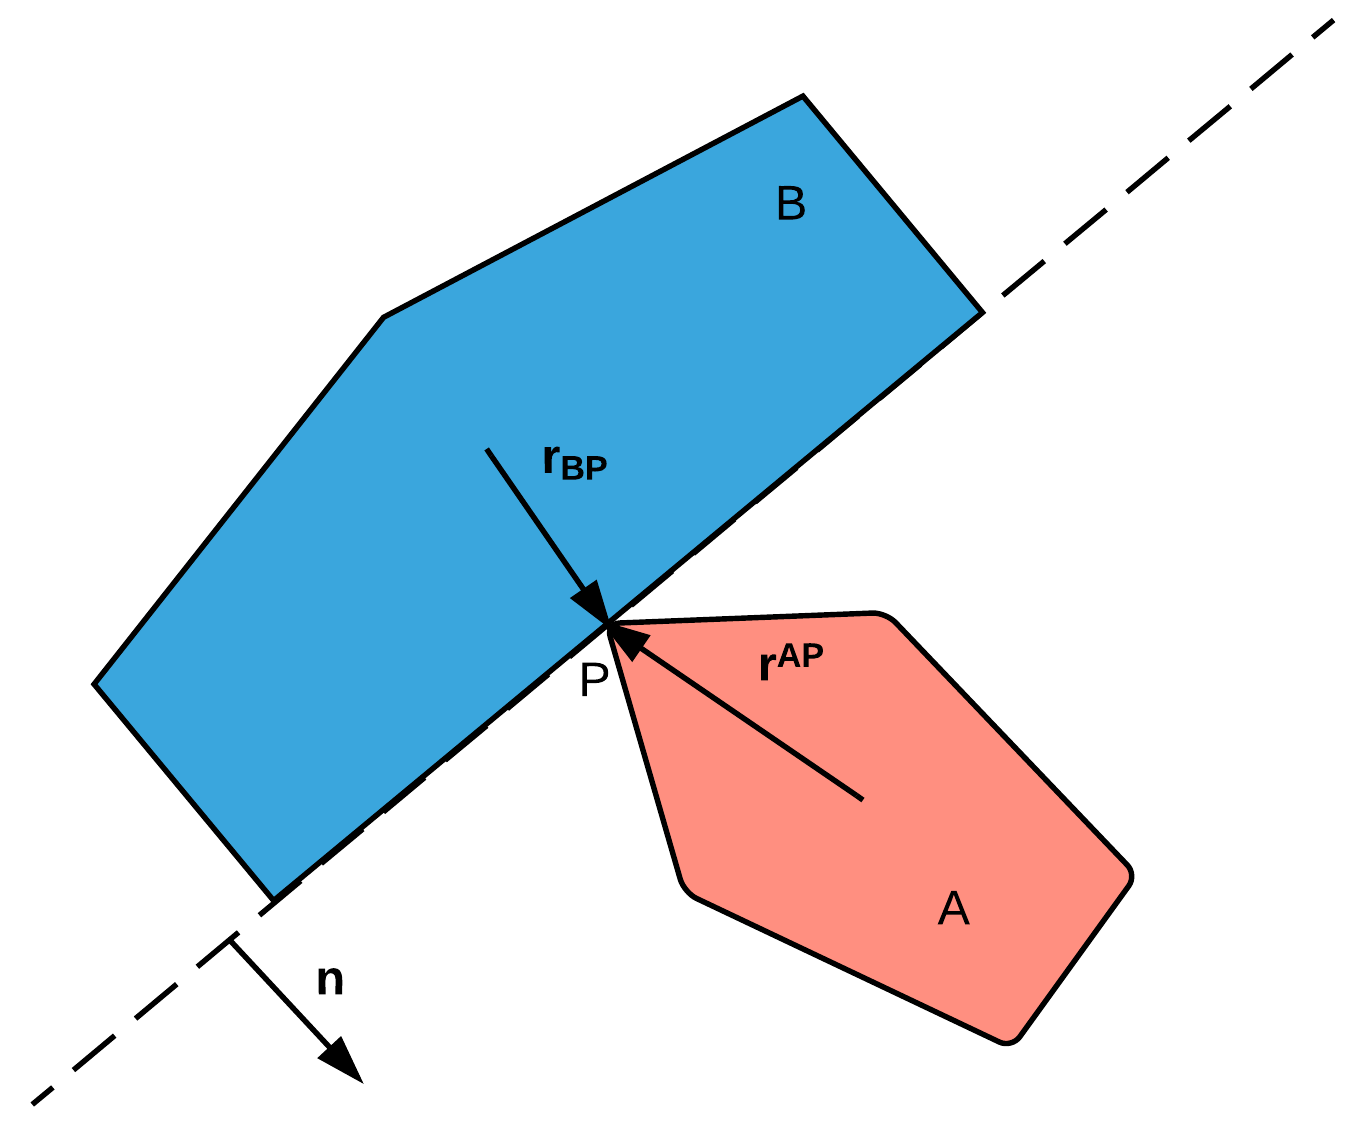
\includegraphics[width=1\textwidth]{CollisionDiagram.png}
		}
		\bigskip
		\caption{\label{Fig_collision}Collision between two rigid bodies}
	\end{center}
\end{figure}

~\newline

%4.2.6 Data Constraints
\subsubsection{Data Constraints} \label{sec_DataConstraints}    

Table~\ref{TblInputVar} and \ref{TblOutputVar} show the data constraints on the input and output variables, respectively.  The ``Physical Constraints" column gives the physical limitations on the range of values that can be taken by the
variable.  The constraints are conservative, to give the user of the model the
flexibility to experiment with unusual situations.  The column of typical values
is intended to provide a feel for a common scenario. 

\renewcommand{\thetable}{1}
%Table of input variables
\begin{table}[!h]
\renewcommand{\arraystretch}{1.2}
\noindent \begin{longtable}{l l l c} 
  \toprule
  \textbf{Var} & \textbf{Physical Constraints} & \textbf{Typical Value} \\
  \midrule 
  $L$ 			& $L\ge0$			&44.2 \si{\metre}
  \\
  $m$			& $m \ge 0$		&	56.2 \si{\kilogram} 
  \\
  $\mathbf{I}$   & $\mathbf{I} \ge 0$ & 74.5 \si{\kilogram\metre\tothe{2}}
  \\
  $g$			& None			& 9.8 \si{\metre\per\second\tothe{2}}	
  \\
  $\mathbf{p}$		& None			& (0.412, 0.502) \si{\metre}	
  \\
  $\mathbf{v}$			 & None 			& 2.51 \si{\metre\per\second}	
  \\
  $C_\text{R}$  	& $ 0 \le C_\text{R} \le 1$	& 0.8 
  \\
  $\boldsymbol \phi$		 & $ 0 \le \phi< 2\pi $	&$\frac{\pi}{2} $ \si{\radian}
  \\	
  $\boldsymbol \omega$ 		& None 			& 2.1 \si{\radian\per\second}
  \\
  $\mathbf{F}$	&	None			& 98.1 \si{\newton}
  \\
  $\boldsymbol{\tau}$ & None		& 200 \si{\newton\metre} 
  \\
  %%%%%%%%%%%%%%%%%%% not included %%%%%%%%%%%%%%%%%%%%%%%%%%%%%%%%%%%
  \iffalse
  $k$			& $k\ge0$			&1.4 \si{\newton\per\metre}
  \\
  $V$ 			& $V>0$ (*)			& 22 \si{\metre^{3}} 
  \\
  $\rho$ 		& $\rho\ge 0$ 		&1 \si{\kilo\gram\per\metre^{3}} 
  \\
  \fi
  \bottomrule
\end{longtable}
\bigskip
\caption{Input Variables} \label{TblInputVar}
\end{table}

\renewcommand{\thetable}{2}
%Table of output variables
\begin{table}[!h]
\renewcommand{\arraystretch}{1.2}
\noindent \begin{longtable}{l l} 
  \toprule
  \textbf{Var} & \textbf{Physical Constraints} \\
  \midrule 
  $\bf p$ 		& None
  \\
  $\bf v$ 		& None
  \\
  $\boldsymbol \phi$	&$ 0 \le \phi< 2\pi $
  \\
  $\boldsymbol \omega$	& None
  \\
  \bottomrule
\end{longtable}
\bigskip
\caption{Output Variables} \label{TblOutputVar}
\end{table}

%%%%%%%%%%%%%%%%%%%%%%%%
%
%	5.) Requirements 
%
%%%%%%%%%%%%%%%%%%%%%%%%

\section{Requirements}

This section provides the functional requirements: the business tasks that the
software is expected to complete, and the nonfunctional requirements: the
qualities that the software is expected to exhibit.

%5.1 Functional Requirements
\subsection{Functional Requirements}

\noindent
\begin{itemize}

\item[R\refstepcounter{reqnum}\thereqnum \label{R_Space}:] Create a space for all of the rigid bodies in the physical simulation 
to interact in.  
\item[R\refstepcounter{reqnum}\thereqnum \label{R_Rigid}:] Input the initial mass, velocities, positions, orientations, angular velocities of, and forces applied on rigid bodies (\iref{IM_FT}, \iref{IM_FR}, \rref{R_CheckInputs}).
\item[R\refstepcounter{reqnum}\thereqnum \label{R_Shape}:] Input the surface properties of the bodies, such as friction or elasticity (\iref{IM_C}, \rref{R_CheckInputs}),
\item[R\refstepcounter{reqnum}\thereqnum \label{R_CheckInputs}:] Verify that the inputs satisfy the required physical constraints (Section \ref{sec_DataConstraints}).
\item[R\refstepcounter{reqnum}\thereqnum \label{R_Force}:] Determine the position and velocities over a period of time of the 2D
rigid bodies acted upon by a force (\iref{IM_FT}).
\item[R\refstepcounter{reqnum}\thereqnum \label{R_Rotation}:] Determine the orientation and angular velocities over a period of time of
the 2D rigid bodies (\iref{IM_FR}).
\item[R\refstepcounter{reqnum}\thereqnum \label{R_CheckCollision}:] Determine if any of the rigid bodies in the space have collided (\rref{R_Space}).
\item[R\refstepcounter{reqnum}\thereqnum \label{R_Collision}:] Determine the position and velocities over a period of time of 2D rigid
bodies that have undergone a collision (\iref{IM_C}, \rref{R_CheckCollision}).

\end{itemize} 

%5.2 Nonfunctional Requirements
\subsection{Nonfunctional Requirements}
Games are resource-intensive, so performance is a high priority.
Other non-functional requirements that are a priority are: correctness,
understandability, portability, reliability, and maintainability. 


%%%%%%%%%%%%%%%%%%%%%%%%
%
%	6.) Likely Changes 
%
%%%%%%%%%%%%%%%%%%%%%%%%

\section{Likely Changes}    

This section lists the likely changes to be made to the physics game library.

\begin{itemize}
	\item[LC\refstepcounter{lcnum}\thelcnum\label{LC_solver}:] The internal ODE-solving algorithm used by the library may change in the future.
	\item[LC\refstepcounter{lcnum}\thelcnum\label{LC_collisions}:] The library may be expanded to deal with edge-to-edge and vertex-to-vertex collisions (A\ref{A_col}).
	\item[LC\refstepcounter{lcnum}\thelcnum\label{LC_damping}:] The library may be expanded to include motion with damping (A\ref{A_damping}).
	\item[LC\refstepcounter{lcnum}\thelcnum\label{LC_constraints}:] The library may be expanded to include joints and constraints (A\ref{A_constraints}).
\end{itemize}


%%%%%%%%%%%%%%%%%%%%%%%%%%%%%%%%%%%%%%%%
%
%	7.) Traceability Matrices and Graphs
%
%%%%%%%%%%%%%%%%%%%%%%%%%%%%%%%%%%%%%%%%

\section{Traceability Matrices and Graphs} \label{sec_tmag}

The purpose of traceability matrices is to provide easy references on what has to be additionally modified if a certain component is changed. Every time a component is changed, the items in the column of that component that are marked with an ``X" should be modified as well. Table \ref{RTraceMatrix} shows the dependencies of goal statements, requirements, instance models and data constraints with each other. Table \ref{ATraceMatrix} shows the dependencies of theoretical models, general definitions, data definitions and instance models on the assumptions. Finally, Table \ref{ITraceMatrix} shows the dependencies of the theoretical models, general definitions, data definitions and instance models on each other. \\

\renewcommand*{\thetable}{3}
\begin{table}[h!]
\renewcommand*{\arraystretch}{1.2}
\centering
\begin{tabular}{|c|c|c|c|c|c|c|c|}
\hline
& \iref{IM_FT} & \iref{IM_FR} & \iref{IM_C} & \rref{R_Space} & \rref{R_CheckInputs} & \rref{R_CheckCollision} & Data Constraints (\ref{sec_DataConstraints}) \\ \hline
\gsref{G_linear}			&X& & & & & & \\ \hline
\gsref{G_angular} 			& &X& & & & & \\ \hline
\gsref{G_detectCollision} 	& & & & & & & \\ \hline
\gsref{G_collision} 		& & &X& & &X& \\ \hline
\rref{R_Space} 				& & & & & & & \\ \hline
\rref{R_Rigid} 				&X&X& & &X& & \\ \hline
\rref{R_Shape} 				& & &X& &X& & \\ \hline
\rref{R_CheckInputs} 		& & & & & & &X\\ \hline
\rref{R_Force} 				&X& & & & & & \\ \hline
\rref{R_Rotation} 			& &X& & & & & \\ \hline
\rref{R_CheckCollision} 	& & & &X& & & \\ \hline
\rref{R_Collision} 			& & &X& & &X& \\ \hline
\end{tabular}
\bigskip
\caption{Traceability Matrix showing the connections between Goal Statements, Requirements, Data Constraints and Instance Models} \label{RTraceMatrix}
\end{table}

\renewcommand*{\thetable}{4}
\begin{table}[h!]
\renewcommand*{\arraystretch}{1.2}
\centering
\begin{tabular}{|c|c|c|c|c|c|c|c|}
\hline 
& \aref{A_rigid} & \aref{A_2d} & \aref{A_cartesian} & \aref{A_right} & \aref{A_col} & \aref{A_damping} & \aref{A_constraints} \\ \hline
\tref{T_NSL} 			& & & & & & & \\ \hline
\tref{T_NTL} 			& & & & & & & \\ \hline
\tref{T_NUG} 			& & & & & & & \\ \hline
\tref{T_CT} 			&X& & & & & & \\ \hline
\tref{T_NRM} 			& & & & & & & \\ \hline
\dref{GD_I} 			& & & & & & & \\ \hline
\dref{GD_COM} 			& & & & & & & \\ \hline
\dref{GD_GA} 			& &X&X& & & & \\ \hline
\dref{GD_RV} 			& & & & & & & \\ \hline
\dref{GD_COR} 			& & & & & & & \\ \hline
\dref{GD_T} 			& & & & & & & \\ \hline
\dref{GD_MI} 			& & & & & & & \\ \hline
\ddref{DD_CM} 			&X&X& & & & & \\ \hline
\ddref{DD_LD} 			&X&X& & & &X& \\ \hline
\ddref{DD_LV} 			&X&X& & & &X& \\ \hline
\ddref{DD_LA} 			&X&X& & & &X& \\ \hline
\ddref{DD_AD} 			&X&X& & & &X& \\ \hline
\ddref{DD_AV} 			&X&X& & & &X& \\ \hline
\ddref{DD_AA} 			&X&X& & & &X& \\ \hline
\ddref{DD_IM} 			&X&X& &X&X& & \\ \hline
\iref{IM_FT} 			&X&X& & & &X&X\\ \hline
\iref{IM_FR} 			&X&X& &X& &X&X\\ \hline
\iref{IM_C} 			&X&X& & &X&X&X\\ \hline
\lcref{LC_solver}		& & & & & & & \\ \hline
\lcref{LC_collisions}	& & & & &X& & \\ \hline
\lcref{LC_damping}		& & & & & &X& \\ \hline
\lcref{LC_constraints}	& & & & & & &X \\ \hline
\end{tabular}
\bigskip
\caption{Traceability Matrix showing the connections between Assumptions and other items} \label{ATraceMatrix}
\end{table}

\begin{landscape}
\renewcommand*{\thetable}{5}
\begin{table}[h!]
\centering\small\setlength\tabcolsep{2.5pt}
\begin{tabular}{|c|c|c|c|c|c|c|c|c|c|c|c|c|c|c|c|c|c|c|c|c|c|c|c|}
\hline
 & \tref{T_NSL} & \tref{T_NTL} & \tref{T_NUG} & \tref{T_CT} & \tref{T_NRM} & \dref{GD_I} & \dref{GD_COM} & \dref{GD_GA} & \dref{GD_RV} & \dref{GD_COR} & \dref{GD_T} & \dref{GD_MI} & \ddref{DD_CM} & \ddref{DD_LD} & \ddref{DD_LV} & \ddref{DD_LA} & \ddref{DD_AD} & \ddref{DD_AV} & \ddref{DD_AA} & \ddref{DD_IM} & \iref{IM_FT} & \iref{IM_FR} & \iref{IM_C} \\ \hline
 \tref{T_NSL} 	& & & & & & & & & & & & & & & & & & & & & & &  \\ \hline
 \tref{T_NTL} 	& & & & & & & & & & & & & & & & & & & & & & &  \\ \hline
 \tref{T_NUG} 	& & & & & & & & & & & & & & & & & & & & & & &  \\ \hline
 \tref{T_CT} 	& & & & & & & & & & & & & & & & & & & & & & &  \\ \hline
 \tref{T_NRM} 	& & & & & & & & & & &X&X& & & & & & & & & & &  \\ \hline
 \dref{GD_I} 	&X& & & & & & & & & & & & & & & & & & & & & &  \\ \hline
 \dref{GD_COM} 	& &X& & & &X& & & & & & & & & & & & & & & & &  \\ \hline
 \dref{GD_GA} 	&X& &X& & & & & & & & & & & & & & & & & & & &  \\ \hline
 \dref{GD_RV} 	& & & & & & & & & & & & & & & & & & & & & & &  \\ \hline
 \dref{GD_COR} 	& & & & & & & & &X& & & & & & & & & & & & & &  \\ \hline
 \dref{GD_T} 	& & & & & & & & & & & & & & & & & & & & & & &  \\ \hline
 \dref{GD_MI} 	& & & & & & & & & & & & & & & & & & & & & & &  \\ \hline
 \ddref{DD_CM} 	& & & & & & & & & & & & & & & & & & & & & & &  \\ \hline
 \ddref{DD_LD} 	& & & & & & & & & & & & & & & & & & & & & & &  \\ \hline
 \ddref{DD_LV} 	& & & & & & & & & & & & & & & & & & & & & & &  \\ \hline
 \ddref{DD_LA} 	& & & & & & & & & & & & & & & & & & & & & & &  \\ \hline
 \ddref{DD_AD} 	& & & & & & & & & & & & & & & & & & & & & & &  \\ \hline
 \ddref{DD_AV} 	& & & & & & & & & & & & & & & & & & & & & & &  \\ \hline
 \ddref{DD_AA} 	& & & & & & & & & & & & & & & & & & & & & & &  \\ \hline
 \ddref{DD_IM} 	& & & &X& &X& & &X&X& &X& & & & & & & & & & &X \\ \hline
 \iref{IM_FT} 	&X& & & & & & &X& & & & &X&X&X&X& & & & & & &  \\ \hline
 \iref{IM_FR} 	& & & & &X& & & & & & & & & & & &X&X&X& & & &  \\ \hline
 \iref{IM_C} 	& & & & & &X&X& & & &X&X&X& & & & & & &X& & &  \\ \hline
\end{tabular}
\bigskip
\caption{Traceability Matrix showing the connections between items of different sections} \label{ITraceMatrix}
\end{table}
\end{landscape}

\noindent
The purpose of the traceability graphs is also to provide easy references on what has to be additionally modified if a certain component is changed. The arrows in the graphs represent dependencies. The component at the tail of an arrow is depended on by the component at the head of that arrow. Therefore, if a component is changed, the components that it points to should also be changed. Figure \ref{Fig_RTrace} shows the dependencies of goal statements, requirements, instance models and data constraints with each other. Figure \ref{Fig_ATrace} shows the dependencies of theoretical models, general definitions, data definitions and instance models on the assumptions. Finally, Figure \ref{Fig_ITrace} shows the dependencies of the theoretical models, general definitions, data definitions and instance models on each other. Building a tool to automatically generate the graphical representation of the matrix by scanning the label and reference can be future work. \\

\begin{figure}[h!]
	\begin{center}
		{
			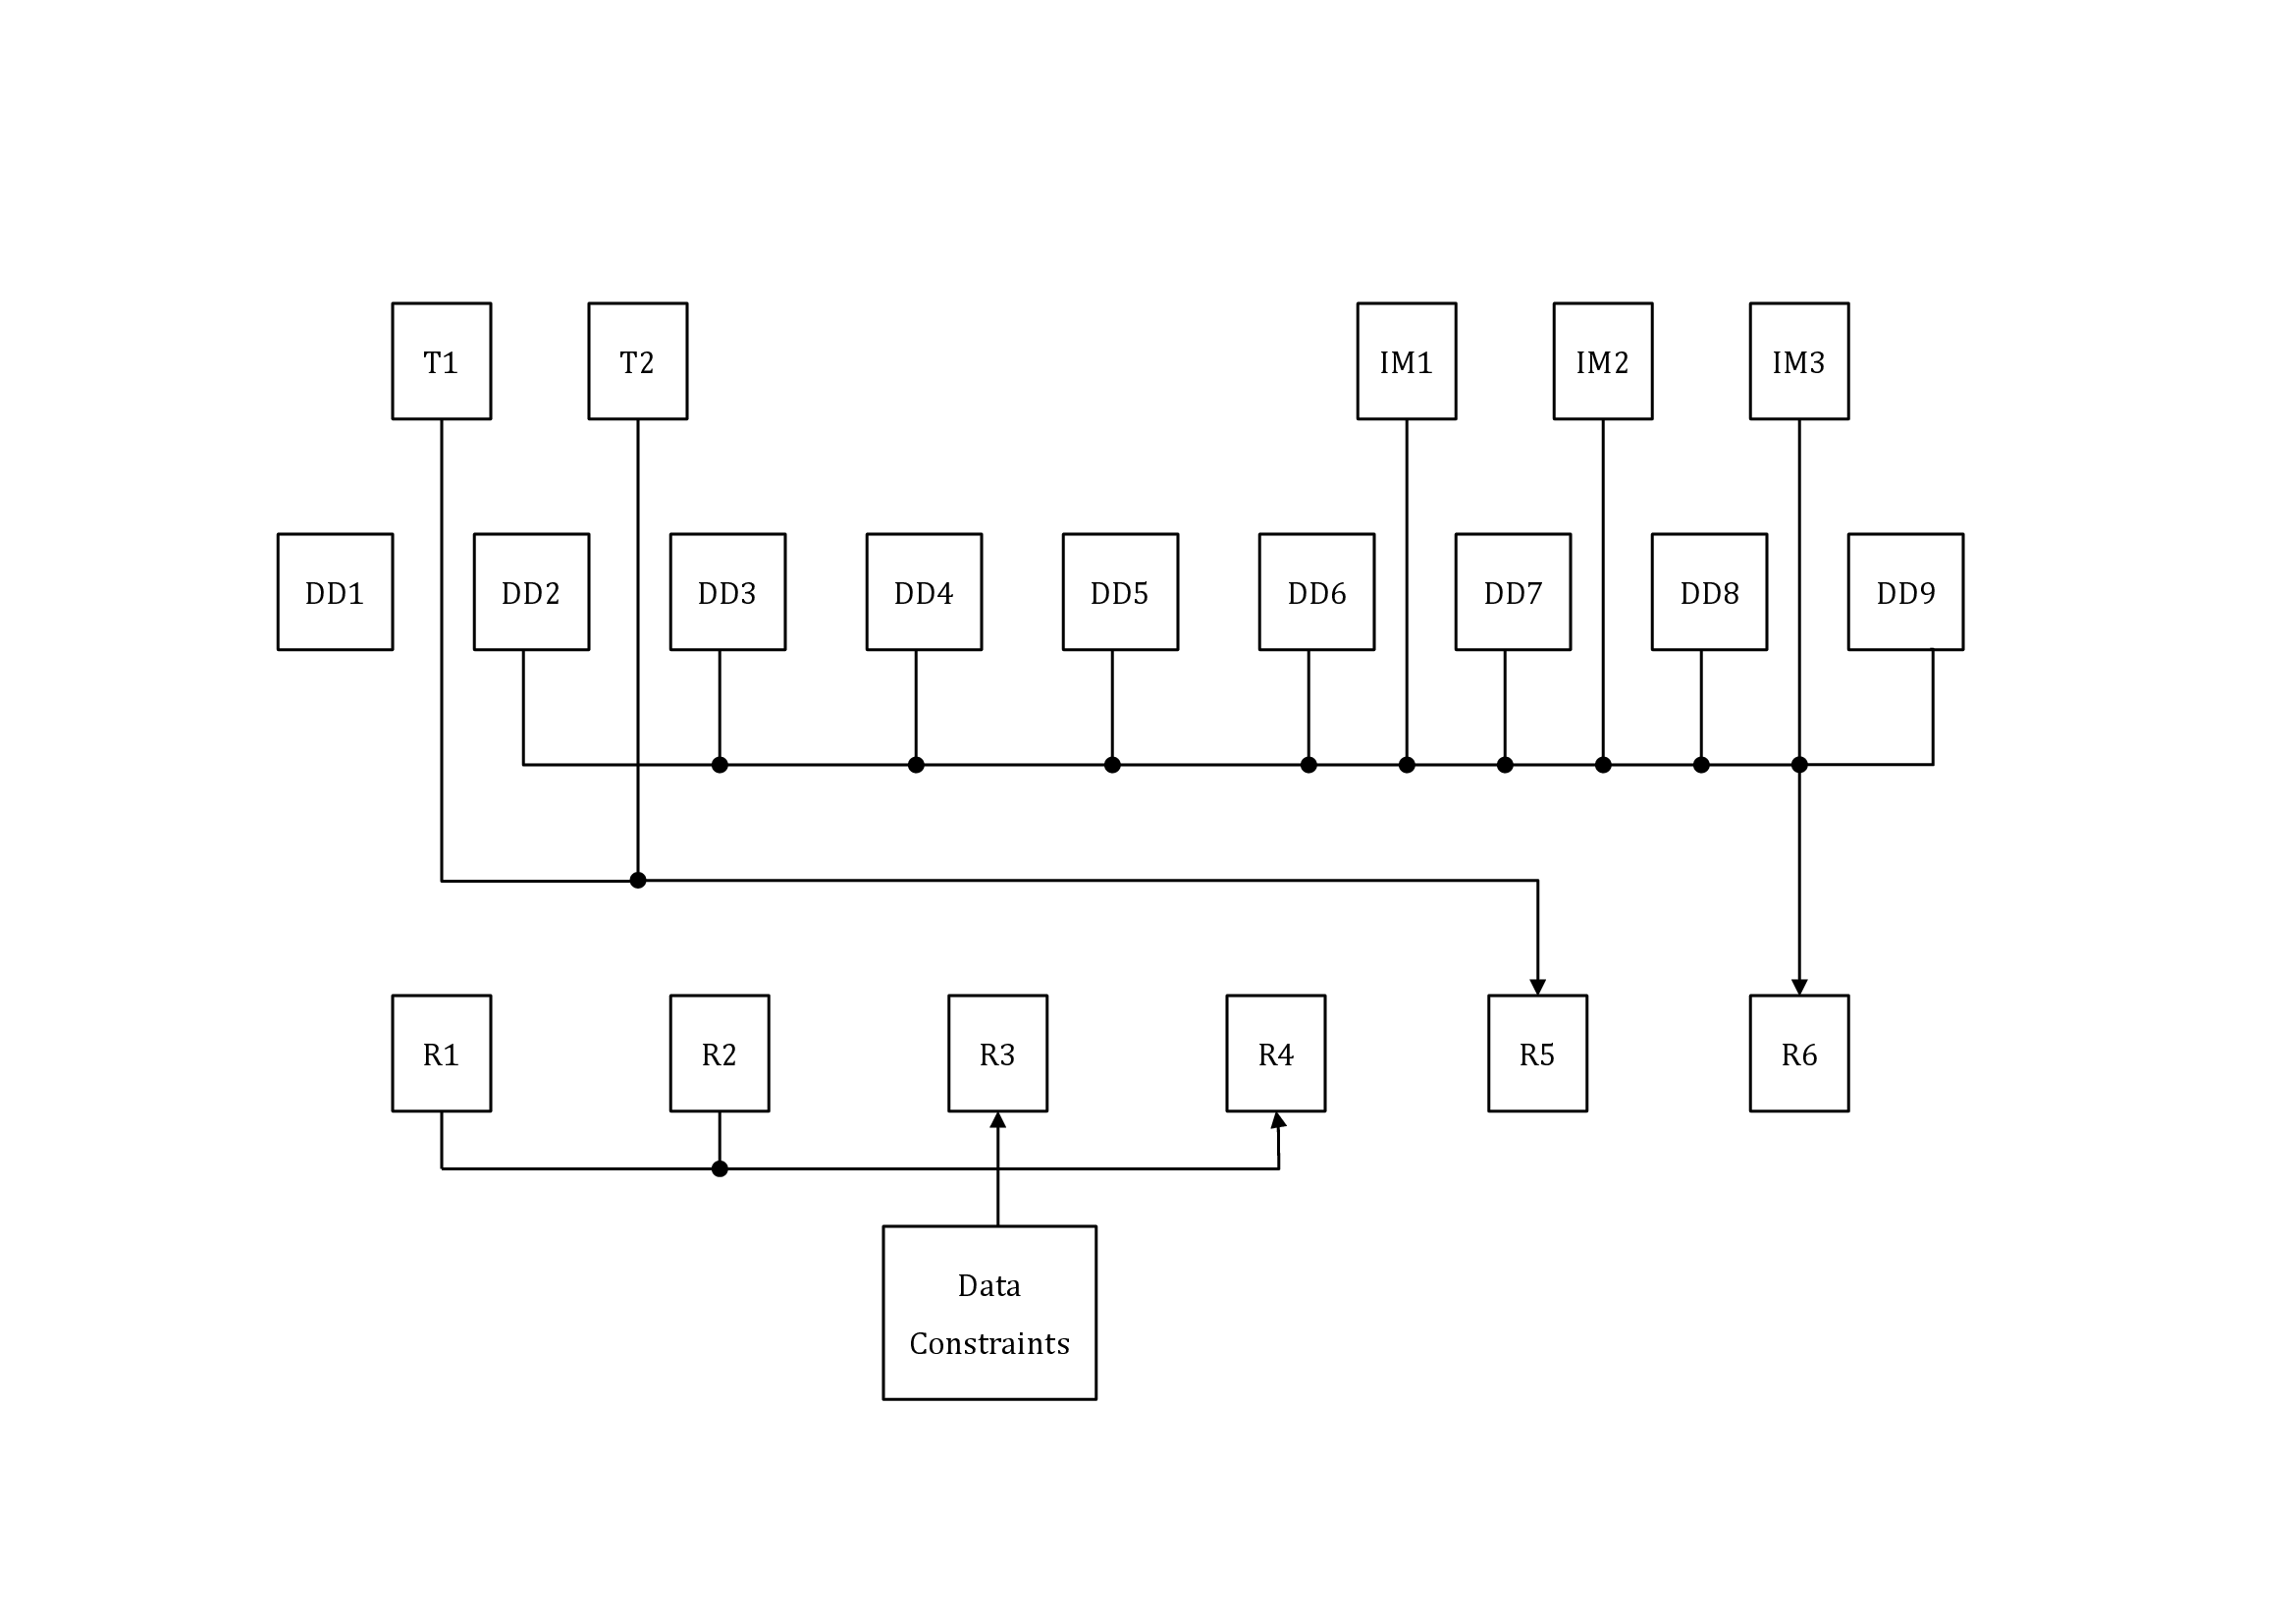
\includegraphics[width=0.8\textwidth]{RTrace.png}
		}
		\bigskip
		\caption{Traceability Graph showing the connections between Goal Statements, Requirements, Data Constraints and Instance Models}
		\label{Fig_RTrace}
	\end{center}
\end{figure}

\begin{figure}[h!]
	\begin{center}
		{
		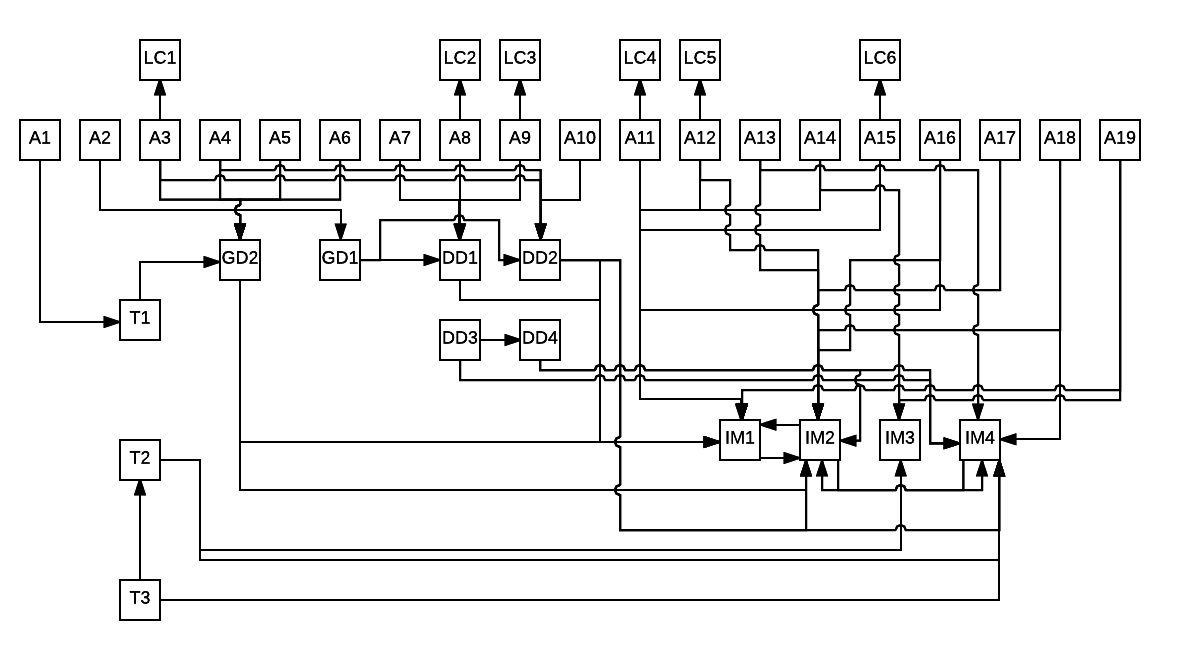
\includegraphics[width=0.71\textwidth]{ATrace.png}
		}
	\bigskip
	\caption{Traceability Graph showing the connections between Assumptions and other items}
	\label{Fig_ATrace}
	\end{center}
\end{figure}

\begin{figure}[h!]
	\begin{center}
		\includegraphics[width=0.71\textwidth]{ITrace.png}
		\bigskip
		\caption{Traceability Graph showing the connections between items of different sections}
		\label{Fig_ITrace}
	\end{center}
\end{figure}

~\pagebreak

%%%%%%%%%%%%%%%%%%%%%%%%%%%%%%%
%
%	8.) Off the Shelf Solutions
%
%%%%%%%%%%%%%%%%%%%%%%%%%%%%%%%

\section{Off the Shelf Solutions}   \label{sec_otss}
As mentioned in section \ref{Sec_pd}, there already exist free open source game
physics libraries. Similar 2D physics libraries are:
\begin{itemize} 
\item Box2D   \url{http://box2d.org/}
\item Nape Physics Engine  \url{http://napephys.com/}
\end{itemize}

\noindent
Free open source 3D game physics libraries include:
\begin{itemize} 
\item Bullet   \url{http://bulletphysics.org/}
\item Open Dynamics Engine  \url{http://www.ode.org/}
\item Newton Game Dynamics  \url{http://newtondynamics.com/}
\end{itemize}

\bibliographystyle {plain}
\bibliography {../Physics_Game_Library}

\end{document}